\documentclass[12pt, openany]{book}

% This is all the packages and settings and so on.
% It is using custom fonts that needs to be installed on the computer. If they are not present, they have to be added manually.
%My additions

\usepackage{unicode-math}



\usepackage[colorinlistoftodos]{todonotes}
\usepackage{cleveref}
\newcommand{\bm}[1]{\symbfit{#1}}
\newcommand{\bmu}[1]{\symbfup{#1}}



\usepackage{polyglossia}

\usepackage[
	citestyle=ieee,
    bibstyle=ieee,
    style=numeric-comp,
    sorting=nty,
    maxbibnames=99, % Make sure we are printing all authors in the appendix
   	backend = biber
    ]{biblatex}

% Makes the last name first in the bibliography.
% \DeclareNameAlias{author}{last-first}
\DeclareNameAlias{author}{family-given}

% Specify the margins. This is 6.25inches in text with which
% can be used to size figures to the correct size.
\usepackage[a4paper, margin=2.5625cm]{geometry}

\usepackage{eso-pic}					% Packages for layout and graphics
\usepackage{graphicx}
\usepackage{tikz}
\usetikzlibrary{fadings}
\usepackage{setspace}
%% \usepackage{tocloft}		 			% Fixing a bug with page style changes for toc
%% \tocloftpagestyle{plain}
\usepackage{etoc} 						% Separate tocs for appendix and the rest
\usepackage{chngcntr}					% Count figures within chapters
\usepackage{booktabs}					% Table formatting
\usepackage{fancyhdr}					% Setting the style for header and footer.
\usepackage{tabularx}
\usepackage{multirow}                   % For better tables
%\usepackage[hidelinks]{hyperref}		% Clickable links
%\usepackage{nameref}					% References with names
\usepackage[parfill]{parskip}			% New line instead of indent for sections
\usepackage{tcolorbox}					% Create boxes around content
\tcbset{colback=white,arc=0mm}
%
%
\usepackage{mathdots}
%%\usepackage{yhmath}
\usepackage{siunitx}
\usepackage{array}
%\usepackage{gensymb}
%%\usepackage{amssymb}
\usepackage{mathtools}              % Add text to math arrows.
%
\usepackage{cancel}
\usepackage{color}
\usepackage{multirow}
\usepackage{textcomp}               % Fixing warning for gensyb \perthousand
\usepackage{svg}                    % including svg files
\usepackage{caption}                % For subfigures
\usepackage{subcaption}
\usepackage{sectsty}
\usepackage{tocloft}

\usepackage[printonlyused]{acronym}




\newcommand{\todi}[1]{\todo[inline]{#1}}
\newcommand{\addref}[1]{\todo[color = yellow]{#1}}
\newcommand{\rewrite}[1]{\todo[color = green]{#1}}



\counterwithin{figure}{section}
\counterwithin{table}{section}

% Specifying fonts
\setmainfont{Georgia}
\setsansfont{Arial}
\newfontfamily\footerfont{Georgia}

\chapterfont{\sffamily\fontsize{17}{17}}
\sectionfont{\sffamily\fontsize{14}{15}}
\subsectionfont{\sffamily\fontsize{13}{15}}
\subsubsectionfont{\sffamily\fontsize{12}{15}}

% Remove the title and make sure that the text is adjusted
% \usepackage{abstract}
% \setlength{\absleftindent}{0mm}
% \renewcommand{\abstractname}{\vspace{-\baselineskip}}
% \renewcommand{\abstractnamefont}{\sffamily\fontsize{14}{15}}
% \renewcommand{\abstracttextfont}{\normalfont\fontsize{12}{13}}

% Renaming and setting style of table of contents
\renewcommand*\contentsname{Contents}
\renewcommand*\cfttoctitlefont{\fontsize{16}{0}\bf\sffamily}
\renewcommand\cftchapfont{\fontsize{14}{0}\bf\sffamily}
\renewcommand\cftchappagefont{\fontsize{13}{0}\bf\sffamily}
\renewcommand\cftsecfont{\fontsize{12}{0}\sffamily}
\renewcommand\cftsecpagefont{\fontsize{12}{0}\sffamily}
\renewcommand\cftsubsecfont{\fontsize{12}{0}\sffamily}
\renewcommand\cftsubsecpagefont{\fontsize{12}{0}\sffamily}

% Styling the header and footer
\fancyhf{}
\fancyhead{}
\fancyfoot{}
\fancyhead[L]{\fontsize{11}{10}\selectfont\leftmark}
\fancyfoot[R]{\footerfont\thepage}
\setlength{\headheight}{15.5pt}


\fancypagestyle{plain}{
    \fancyhf{}
    \fancyhead{}
    \fancyfoot{}
    \renewcommand{\headrulewidth}{0pt}
    \fancyfoot[R]{\footerfont\thepage}
}

\pagestyle{fancy}

% Making the command for placing text in random locations
\newcommand\PlaceText[3]{%
\begin{tikzpicture}[remember picture,overlay]
\node[outer sep=0pt,inner sep=0pt,anchor=south west]
  at ([xshift=#1,yshift=-#2]current page.north west) {#3};
\end{tikzpicture}%
}

% Disable hyphenation
\pretolerance=10000
\tolerance=2000
\emergencystretch=50pt


% Defining files for bibliography
%\addbibresource{ref.bib}
\addbibresource{references.bib}
% Add a second bibliography file for the second author to allow
% both to update it through the mendeley integration.
% \addbibresource{ref-author-2.bib}

% Defining document information
\title{Template}
\newcommand{\subtitle}{KTH Thesis Report}
\author{Max Schaufelberger}

\begin{document}
\setstretch{1.4}

% The front page of the document
\pagenumbering{roman}
\makeatletter
\begin{titlepage}

\vspace*{-4.6\baselineskip}
\hspace*{-0.15\textwidth}
\includegraphics[width=0.2\paperwidth]{setup/img/kth-logo.jpg}
\par\vspace*{2.5\baselineskip}

\PlaceText{65mm}{12mm}{\fontsize{12}{0}\sffamily DEGREE PROJECT IN TECHNOLOGY,}
\PlaceText{65mm}{17mm}{\fontsize{12}{0}\sffamily SECOND CYCLE, 30 CREDITS}
\PlaceText{65mm}{22mm}{\fontsize{12}{0}\sffamily\itshape STOCKHOLM, SWEDEN \the\year}

~\\

\makebox[0pt][l]{%
\begin{minipage}[b]{0.25\textwidth}
~\\
\end{minipage}
\begin{minipage}{0.65\textwidth}
\begin{flushleft}
{\fontsize{28}{24}\bf\sffamily\@title\\}
\vspace{1cm}
{\fontsize{19}{17}\bf\sffamily \subtitle\\}
\vspace{1cm}
{\fontsize{16}{18}\sffamily \@author}\\
\end{flushleft}
\end{minipage}
}


% \hspace*{-3cm}\begin{minipage}[b]{63.5mm}
% ~\\
% \end{minipage}
% \begin{minipage}{0.65\textwidth}
% \begin{flushleft}
% {\fontsize{28}{24}\bf\sffamily\@title\\}
% \vspace{0.5cm}
% {\fontsize{19}{17}\bf\sffamily \subtitle\\}
% \vspace{0.5cm}
% {\fontsize{16}{0}\sffamily \@author}\\
% \end{flushleft}
% \end{minipage}


\AddToShipoutPictureBG*{%]
    \AtPageLowerLeft{%
        
\includegraphics[width=1.0\paperwidth]{setup/img/kth-footer.png}
    }%
}

\PlaceText{70mm}{280mm}{\color{white}\fontsize{12}{0}\sffamily KTH ROYAL INSTITUTE OF TECHNOLOGY }
\PlaceText{70mm}{285mm}{\color{white}\fontsize{8}{0}\sffamily SCHOOL OF ENGINEERING SCIENCES}
\end{titlepage}
\makeatother

\newpage
\newpage
\thispagestyle{plain}
~\\
\vfill
{ \setstretch{1.1}
	\subsection*{Author}
	Max Schaufelberger <maxscha@kth.se>\\
	School of Engineering Sciences\\
	KTH Royal Institute of Technology

	\subsection*{Place for Project}
	Stockholm, Sweden\\
	Ottignies-Louvain-la-Neuve, Belgium

	\subsection*{Examiner }
	Prof. Elias Jarlebring\\
	Department of Numerical Analysis\\
	KTH Royal Institute of Technology\\
	Stockholm, Sweden
	~
	\subsection*{Supervisor }
	Arvind Kumar\\
	Division of Computational Science and Technology\\
	KTH Royal Institute of Technology\\
	Stockholm, Sweden
	~
	\subsection*{Supervisor }
	Frédéric Crevecoeur\\
	Institute of Information and Communication Technologies, Electronics and Applied Mathematics\\
	UCLouvain Catholic University of Louvain\\
	Louvain-la-Neuve, Belgium
	~


}


\newpage
\thispagestyle{plain}
%%%%%%%%%%%%%%%%%%%%%%%%%%%%%%%%%%%%
%%  The English abstract          %%
%%%%%%%%%%%%%%%%%%%%%%%%%%%%%%%%%%%%
\chapter*{Abstract}
%%%%%%%%%%%%%%%%%%%%%%%%%%%%%%%%%%%%

%This is a template for writing thesis reports for the ICT school at KTH. I do not own any of the images provided in the template and this can only be used to submit thesis work for KTH.

The emergence of spiking networks as the third generation of neural networks has shown great success in solving various tasks. Here, networks of spiking neurons are used to control a linear system using biologically plausible methods. Spiking neurons are introduced, and different frameworks highlighted. The control concept consists of two efficient coding networks: one for generating the necessary input to drive the second network, simulating the dynamics. The precise network behaviour is explained using a geometric methods. Network parameters for the simulating network are learned using supervised and unsupervised learning rules.\\
For the simulation, results from the spiking network are accurate for various system sizes.\\
Applying the control network to the dynamic system directly, independent of the simulating network, yields valid results as long as conditions on the input and output matrices are met.\\
Acceptable results for control using two networks can be reached if either the learning or the input matrix of the problem is neglected.\\
Control using learned matrices is limited by inaccuracies in the supervised learning of matrix parameters as well as problem-dependent tuning of hyper-parameters. Moreover, learning progress is hard to monitor without repeated testing by simulation.\\
The results of this thesis suggest that the methods are unable to capture a general black box problem of designing a controller but can be useful when additional information is available.


\subsection*{Keywords}
Spiking networks, Control, Efficient Coding Networks, Learning



\newpage
\thispagestyle{plain}
%%%%%%%%%%%%%%%%%%%%%%%%%%%%%%%%%%%%
%%	 The Swedish abstract         %%
%%%%%%%%%%%%%%%%%%%%%%%%%%%%%%%%%%%%
\chapter*{Abstract}
%%%%%%%%%%%%%%%%%%%%%%%%%%%%%%%%%%%%
Framväxten av spikande nätverk som den tredje generationen av neurala nätverk har visat sig vara mycket framgångsrik när det gäller att lösa olika uppgifter. Här används nätverk av spikande neuroner för att styra ett linjärt system med hjälp av biologiskt trovärdiga metoder. Spikande neuroner introduceras och olika ramverk belyses. Kontrollkonceptet består av två effektiva kodningsnätverk: ett för att generera den input som krävs för att driva det andra nätverket, som simulerar dynamiken. Det exakta nätverksbeteendet förklaras med hjälp av geometriska metoder. Nätverksparametrarna för det simulerande nätverket lärs in med hjälp av regler för övervakad och oövervakad inlärning.
För simuleringen är resultaten från spiking-nätverket exakta för olika systemstorlekar.\\
Att tillämpa kontrollnätverket direkt på det dynamiska systemet, oberoende av simuleringsnätverket, ger giltiga resultat så länge villkoren för in- och utgångsmatriserna är uppfyllda.\\
Acceptabla resultat för styrning med två nätverk kan uppnås om antingen inlärnings- eller indatamatrisen för problemet försummas.\\
Styrning med hjälp av inlärda matriser begränsas av felaktigheter i den övervakade inlärningen av matrisparametrar samt problemberoende inställning av hyperparametrar. Dessutom är det svårt att övervaka inlärningsförloppet utan upprepade tester genom simulering.
Resultaten i denna avhandling tyder på att metoderna inte kan fånga ett generellt black box-problem med att utforma en regulator men kan vara användbara när ytterligare information finns tillgänglig.

\subsection*{Nyckelord}
Spikande nätverk, kontroll, Efficient Coding networks, lärande

\newpage
\thispagestyle{plain}
\chapter*{Acknowledgements}


I would like to express my sincere gratitude to my supervisors, Arvind Kumar and Elias Jarlebring, for their invaluable guidance, support, and encouragement throughout the research and writing of this thesis. Their expertise and constructive feedback have been instrumental in shaping the quality and direction of this work.

I am deeply appreciative of the time and effort they devoted to providing insightful suggestions and helping me navigate the challenges of this project.

In conclusion, I extend my sincere appreciation to Arvind Kumar and Elias Jarlebring for their unwavering support and mentorship. Their guidance has been instrumental in making this research endeavour a rewarding and successful experience.

\newpage

\chapter*{Acronyms}

\begin{acronym}[RDBMS]

\acro{DS}{Dynamic System}
\acrodefplural{DS}{Dynamic Systems}

\acro{NN}{Neural Network}
\acrodefplural{NN}{Neural Networks}

\acro{ANN} {Artificial Neural Network}
\acrodefplural{ANN}{Artificial Neural Networks}

\acro{SNN}{Spiking neural network}
\acrodefplural{SNN}{Spiking neural networks}


\acro{ACID}{atomicity, consistency, isolation, and durability}
\acro{CAP}{Consistency, Availability, Partition-tolerant}
\acro{CDF}{Cumulative Distribution Function}
\acro{CPU}{Central Processing Unit}
\acro{IF}{Integrate and Fire}
\acro{LIF}{Leaky-integrate-and-fire}
\acro{RHS}{Right Hand Side}
\acro{HH}{Hodgkin–Huxley}
\acro{NLP}{Natural Language Processing}
\end{acronym}




\newpage

\etocdepthtag.toc{mtchapter}
\etocsettagdepth{mtchapter}{subsection}
\etocsettagdepth{mtappendix}{none}
\thispagestyle{plain}
\tableofcontents

\newpage




\pagenumbering{arabic}

\chapter{Introduction}

Provide a general introduction to the area for the degree project. Use references!

Link things together with references. This is a reference to a section: \ref{sec:background}.

\rewrite{Neuro stuff, very rapid development, tremendous progress, many things are successful with NNs. Then list fields that work well. E.g pattern recognition, bioinformatics, neuroscience. With spiking neural networks they are behind the state of the art feedforward networks but the gap is closing. There are already fields where they are excel compared over normal NN.}


The human brain is a brilliant computing unit comprised of around 86 billion\cite{azevedo_equal_2009} neurons. Each of these neurons can have thousands of connections to other neurons.\addref{Maybe put some exact numbers here and a source}. Between these connections, information travels trough the network as electrical impulses that interact with the neurons own electrical potential. The huge network complex of the human brain is capable of vastly different and intricate tasks.\rewrite{Sounds vague} Some problems that are still next to impossible to solve by machines and classical algorithms alone. Moreover many machine implementations lack the speed, precision or flexibility of the human counterpart.\\
Researchers want to remedy this by mimicking the brain's internal network structure to solve problems deemed unsuitable for classic algorithms.\\
A variety of different architectures have been proposed, with the most prevalent design being a feed-forward network. Information travels only in one direction and is not propagated by spikes but gradients usually set in $[0,1]$ or $[-1,1]$.
These \acp{ANN} have made impressive progress in the fields of image recognition and \ac{NLP}(using Transformers)\addref{Ref for Transformers}\addref{Find some more fields with source!}.\\
This abstract representation bears advantages e.g in modelling and implementation but also gives away some key features of the human brain. Do to the information traveling only towards the output, feed-forward networks cannot build a memory or temporal data. Recurrent models exist which allow for memory \addref{cite some LSTM networks} and sequential data input but loose some of the advantages compared to the Feed-Forward.\\
A third generation of network architectures has risen, which aims to be even more biologically plausible. Inspired from nature, they implement spiking behaviour and recurrence found in the human brain.
This newer form of \ac{SNN} is as powerful as the classic feed-forward but suited for temporal data.\\
While feed-forward networks are still outperforming \acp{SNN}, in some cases \acp{SNN} are on par or more performant\addref{Say smth where they are better with ref}.

\todi{Now list the goal: We want to do it for DS and check how good they are. Then method and then work. Take from below}


Human brain amazing\\
We struggle to make to replicate at the computer level with algorithms\\
Neural network a way to imitate the brain and its inner workings.\\
Neural networks have shown and proven performance in certain areas\\
They lack in some others\\
Therefore considerable research went into it\\
Now we have spiking neural networks, that imitate the brain even more\\
We hope that with that we have even better performance\\
From very biological to very abstract there have been many proposals\\
Cost performance trade off.\\
Spiking networks have gained similar or exceeding performance compared to the artificial one in some areas-> refs\\
Key advantage is in the temporal dimensional gain.\\
One field they are suited well is the control of dynamic systems\\
In this thesis we use a spiking neural network to control a linear dynamic system\\
The usual way to simulate biological dynamic systems is using LQG control -> ref\\
I believe because of the energy minimization\\
So we can compare them with usual NN and control in terms of performance... i guess\\
We start by giving an intro into spiking neural networks\\
Then spiking neural networks for dynamic systems\\
After control theory with SNN and maybe regular LQG control\\
Lately the learnign of SNNs for the control of dynamic system\\

Further work:\\
Maybe learning methods to control nonlinear dynamic systems\\
Maybe we can even do the adverserial attack to try to screw with the network.\\
Implement this on neuromorphic hardware\\

Problem:\\
Problem is that it is unnatural for classic NN to use temporal data.\\
They usually quantize it and make a big input layer -> ref\\
There are recurrent networks but ... they need to have smth bad as well\\
The LQG control is also not great for some reason I need to find\\
There are many spkiking network archetypes like poisson and GLm and balanced\\
Also problem is that for some spiking networks learning rules could be hard to come by.\\
There are many prospects though as for example ......->refs\\
Also usually learning rules smth of an inverse and that the brain does not have or do I believe arvind said\\



Method:\\
We use a SNN to to control any arbitrary DS\\
Balanced networks show a some key motives seen in the brain like poisson distribution and smth else ->ref\\
The SNN is to be trained with a STDP rule\\
Then compared to optimal weights\\
Then investigated about robustness and other things as many before\\
One part of robustness is trying to get the most essential nodes of the snn to function well.\\¸
Then we have the potential to find a classic nn and train it with that ???\\
With that out of the way we can compare the performance of all the methods.\\
Then we could study the usability for biological interpretation.\\
Maybe even train time over performance or smth whatever\\


Work:\\
Explain the controller method aka what the math of the controller\\
In method explain the balanced and the derivation\\
In work summarize the implementation\\
Same for the conventional NN\\
Summarize the training method\\
Explain and derive the training method in method\\


Results:\\
To everthign mentioned in method for performance and so on\\
Answer the questions of the problem!!!!\\


\section{Background}
\label{sec:background}
Present the background for the area. Give the context by explaining the parts that are needed to understand the degree project and thesis. (Still, keep in mind that this is an introductory part, which does not require too detailed description).

Use references\footnote{You can also add footnotes if you want to clarify the content on the same page.}

Detailed description of the area should be moved to Chapter 2, where detailed information about background is given together with related work.


This background presents background to writing a report in latex.


Example citation \cite{Jones2017} or for two authors: \cite{Jones2017, Liu2017}

Look at sample table \ref{tab:sample-table-label} for a table sample.

\begin{table}[!ht]
\centering
\caption{Sample table. Make sure the column with adds up to 0.94 for a nice look.}
~\\
\label{tab:sample-table-label}
\begin{tabular}{p{0.3\textwidth} p{0.64\textwidth}}
\toprule
\textbf{SAMPLE}		  & \textbf{TABLE}                                                                                                                                                  \\ \toprule
One                   & Stuff 1 \\
\midrule
Two                   & Stuff 2 \\
\midrule
Three                 & Stuff 3\\
\bottomrule
\end{tabular}
\end{table}



Boxes can be used to organize content

\begin{tcolorbox}[title={Development environment for prototype}]
	\tt{
		\textbf{Operating systems }\\
		computer: Linux - kernel 4.18.5-arch1-1-ARCH\\
		android phone: 8.1.0\\
		~\\
		\textbf{Build tools}\\
		exp (build tool): version 55.0.4\\
		~\\
		...
	}
\end{tcolorbox}

\section{Problem}
NN have excelled at many fields\\
Fields where they are not fit\\ aka temporal data\\
They have ways to compromise on that \\ -> reference\\
Spiking nn inherently temporal \\
more natural choice\\
However they also have problems\\
like the following:::: reference!!\\
\section{Purpose}
The purpose of the degree project/thesis is the purpose of the written material, i.e., the thesis. The thesis presents the work / discusses / illustrates and so on.

It is not “The project is about” even though this can be included in the purpose. If so, state the purpose of the project after purpose of the thesis).

Probably delete as a own paragraph but mention smth like that.

\section{Goal}
The goal means the goal of the degree project. Present following: the goal(s), deliverables and results of the project.\\

The goal of this project is to create a \ac{SNN} that can control \rewrite{give exact specifications. For example controllability} any given linear \ac{DS}. Furthermore should the \ac{NN} be robust against failing neurons or connections to some degree. With this we can investigate to find the smallest \ac{SNN} with acceptable performance.
Its performance should be comparable or supersede conventional control systems, like \ac{LQG} control, or \acp{NN}. We expect better results to conventional \acp{NN} because of the \ac{SNN}'s natural way to use temporal data. For the \ac{SNN} itself we desire similarities to the brain, such as high precision or Poisson distributed spiking.\addref{What do we else want like the brain.Maybe low spike count? And what can we do?  Also References!}
To mimic the brain's learning, we want to use local training rules that are biologically plausible. The network should be converge to the optimal parameters.\rewrite{This is even more to ask than from a conventional NN, Say in method bcs there it has already been proven if I am not mistaken}. This requirement would allow us to give a justified measure on how close we are replicating the brain's control power compared to our artificial implementation in specific circumstances\rewrite{sounds vague}.

\section{Benefits, Ethics and Sustainability}
Describe who will benefit from the degree project, the ethical issues (what ethical problems can arise) and the sustainability aspects of the project.

Use references!

\section{Methodology}
Introduce, theoretically, the methodologies and methods that can be used in a project and, then, select and introduce the methodologies and methods that are used in the degree project. Must be described on the level that is enough to understand the contents of the thesis.

Use references!

Preferably, the philosophical assumptions, research methods, and research approaches are presented here. Write quantitative / qualitative, deductive / inductive / abductive. Start with theory about methods, choose the methods that are used in the thesis and apply.


Detailed description of these methodologies and methods should be presented in Chapter 3. In chapter 3, the focus could be research strategies, data collection, data analysis, and quality assurance.


We build a SNN for a control problem and check it for performance as mentioned above. In addition we design a conventional controller and compare the result. IF we have the time for it we put a conventional NN to it too. We see the performance compared to the others and look at the specs we mentioned above.
The SNN is trained by learning using STDP rule. We can compare the learned weights with the optimal weights when we have our own optimal controller/ we simulate our trajectory.
For our approach we use a balanced spiking network.
\section{Stakeholders}
Present the stakeholders for the degree project.

\section{Delimitations}
Explain the delimitations. These are all the things that could affect the study if they were examined and included in the degree project.
Use references!

\section{Outline}
In text, describe what is presented in Chapters 2 and forward. Exclude the first chapter and references as well as appendix.

\chapter{<Theoretical Background>}
% \thispagestyle{fancy}
In this chapter, a detailed description about background of the degree project is presented together with related work. Discuss what is found useful and what is less useful. Use valid arguments.

Explain what and how prior work / prior research will be applied on or used in the degree project /work (described in this thesis). Explain why and what is not used in the degree project and give valid reasons for rejecting the work/research.

Use references!

\section{Use headings to break the text}
Do not use subtitles after each other without text in between the sections.

\section{Related Work}
You should probably keep a heading about the related work here even though the entire chapter basically only contains related work.

Here just what has been done for each of the headlines\\
Previous efforts were already made to control dynamic systems with \acp{SNN}.
\todi{List here also efforts with other concepts apart from Balanced Networks}




Neural networks in general
spiking neural networks and their differences and what they are better for.
neuron models, iwazishi neuron and maybe one more
mein neuron model und warum ich es ausgewaelt habe: einfach zu implementieren. Bereits fuer dynamische systeme verwendet,
Nachteile dieses modells.
Vlt vergleich mit einem anderen modell.
Ganz kurzer ausflug in die regelung von dynamischen systemen.


What is a neural network? -> not here ref a paper. kurze erkl'rung in der einfuerung
in der einfuhurng vlt auch hodgekin huxley erwaehen :)



\section{Dynamic systems}

\section{Neuron model}

\subsection{Biological Neuron model}
The most biologically accurate model of neuron spiking is the \ac{HH} model. The \ac{HH}-model considers the neuron with its ion channels. The membrane acts as a capacitance and the travelling ions in each ion channel contribute a current to the overall membrane potential. These ion gates are voltage dependent and are defined positive in direction out of the cell.\\
A particular ion channel for ion $X$ can be modelled as
\begin{equation}
	I_X= g_X \cdot (V-V_X)
\end{equation}
These currents are summed summed for the different ion channels in question, most commonly for Sodium, Potassium and a leak current. In reality there are a plethora of different channels and channel properties\footnote{See  \url{channelpedia.epfl.ch} for an extensive list}. The $V_X$ are the equilibrium potentials for each of the channels and can be computed using the Nernst equation \cite{johnston_foundations_1995}. \addref{Add a reference to a monography.}
\begin{equation}
	C \frac{dV}{dt} = g_{Na} \cdot (V-V_{Na}) + g_K \cdot (V-V_K) + g_l \cdot (V-V_l)
\end{equation}
Do model the voltage dependency of the ion channels, the conductances are described with gating variables, usually called $n$, $h$ and $g$ for Na-Activation, Na-Inactivation and K-activation respectively. One gating variable is set between $[0,1]$ and models the permeability of said gate. Multiple gates are used to fit to each ion channel in order to match experimental data and the model behaviour.\\
Gates have first order dynamics of the form
\begin{equation}
	\frac{dn}{dt} = \alpha_n(1-n) - \beta_n n
\end{equation}
for e.g the n gate. The other gates' dynamics are analogous. The functions $\alpha$ and $\beta$ are voltage but not time dependent. The discussion of initial values as well as functions for $\alpha_p,\ \beta_p\ \ p = (n,h,m)$ can be found in \cite{hodgkin_quantitative_1952} or \cite{johnston_foundations_1995}. The gates for each ion channel's conductance are found to be
\begin{equation}
	\begin{aligned}
	g_{Na} &= \bar{g}_{Na} n^4\\
	g_{K} &= \bar{g}_{K} m^3h\\
	\end{aligned}
\end{equation}
and give form to the final model
\begin{equation}\label{eq:HH}
	\begin{aligned}
	C\frac{dV}{dt} &= I(t) -\bar{g}_{Na} n^4(V-V_{Na}) - \bar{g}_{K} m^3h(V-V_{K}) -g_L(V-V_{L})\\
	\frac{dn}{dt} &= (1-n)\alpha_n(V) - \beta_n n (V)\\
	\frac{dm}{dt} &= (1-m)\alpha_m(V) - \beta_m m (V)\\
	\frac{dh}{dt} &= (1-h)\alpha_h(V) - \beta_h h (V)
	\end{aligned}
\end{equation}
We did not define a gate for the leak term as it is assumed constant.
\subsection{"IF and LIF"}
In contrast of the \ac{HH} model in \cref{eq:HH}, the simplest models of neurons are the \ac{IF} and \ac{LIF} models.\\
\paragraph{IF Neurons}
\ac{IF} Neurons, as the name implies, integrate the incoming current over time.
\begin{equation}
	\frac{d V(t)}{d t} = \frac{1}{C}I(t)
\end{equation}
The membrane voltage is governed by the incoming current spikes of connected neurons and the membrane capacitance. The neuron potential does not change without a change of input current and thus presents as a perfect integrator of the input.\\
\paragraph{\ac{LIF} Neurons}
In contrast to that the \ac{LIF} neuron contains a leak term on the RHS which brings the voltage back to its resting potential over time. The model can be expressed as
\begin{equation}
	\tau\frac{dV(t)}{dt} = -(V(t)-E_r) + RI(t),
\end{equation}
where $\tau = RC$ is the time constant the composed of the membrane resistance $R$ and the membrane capacitance $C$ and the resting potential $E_r$. In the absence of input $I(t)$ the voltage settles on the membrane potential $E_r$.\\
The input $I(t)$ encapsulates external inputs as well as a sum of Dirac functions indicating a spiking neuron
\begin{equation}
	I(t) = \sum_k \delta(t-t^k)
\end{equation}
\rewrite{This is not truly correct. Forgot weights, but at the same time only when there are more than 1 neuron}
and $t_k$ being the time of the $k$-th spike. When the membrane voltage exceeds the threshold potential $\bar{v}$, a spike is sent out by the neuron and the voltage sets back to its reset voltage $v_{res}$.
\subsection{Izhikevich Neuron}
While the above models deliver a useful and cheap simplification, they lack in accuracy. The Izhikevich model \cite{izhikevich_simple_2003} of the neuron tries be the of both worlds in terms of efficiency and accuracy. It is comprised of 2D ODEs with the membrane potential $v$ as
\begin{equation}
	\begin{aligned}
	\frac{d v}{dt} &= 0.04v^2 + 5v + 140 -u +I(t)\\
	\frac{d u}{dt} &= a(bv-u).
	\end{aligned}
\end{equation}
With the chosen factors, the neuron experiences a spike when $u\geq30 $mV, in which case the neuron resets to
\begin{equation}
\begin{aligned}
	u &\leftarrow u+d\\
	v&\leftarrow c
\end{aligned}
\end{equation}
The parameters describe $a$ scale of recovery, $b$ sensitivity, $c$ the reset potential of $v$ and $d$ the reset of variable $u$.\rewrite{Maybe shitty explanation, which could be extended on.} Depending on these parameters one can achieve different behaviours of the neuron e.g. regular spiking, fast spiking and low threshold spiking to name a few \cite{izhikevich_simple_2003}.

\section{Neural Networks}

\subsection{Biological Neural Network}

\subsection{Artificial Neural Networks}
 \todo{Make clear distinction between forward nns and ann. Bcs apparently they are not the same!}
\subsection{Spiking Neural Networks}
A spiking Neural network is one step closer to a biologic representation of a brain. Instead of conveying information using a gradient in conventional \ac{NN}s, information is propagated using discrete spikes of excitation, similar to biological neurons. Hereby one can distinguish between several ideas of implementation.

\subsection{Poisson-Networks}

\subsection{Liquid state machines}
\todi{write how the offline computing is pretty bad for brain things, but good for chess for example. The online computing is what the brain does and it is not yet as developed. add the TU graz paper to refs and some of it's references too, for example nr. 19}
One alternative method has been the use of \ac{LSM} or more general Reservoir computing.\\
The term Reservoir computing was introduced by Benjamin Schrauwen and describes a general group of recurrent network approach\cite{verstraeten_experimental_2007}.\\
The "reservoir" is a non-linear map from input to outputs that combines the input in various, even random ways. These contain but are not limited to sums, differences, multiplications, division and exponentiation. In general the output $\bmu{x}(t)$ is higher dimensional that the input $\bmu{v}(t)$, in order to allow for sufficient variety in the mapping. The output of the reservoir, which is usually treated as a black box, is fed in a linear decoder in order to retrieve the desired output signal.\\
\begin{figure}
	\centering
	\includesvg[scale= 0.15]{reservoir_computing}
	\caption{Abstract idea of Reservoir Computing. Adapted from \cite{cooper_liquid_2011}}
	\label{fig:reservoir_computing}
\end{figure}
The liquid can be made of any system that fulfils two properties.\\
\begin{itemize}
	\item Non-linear nodes of computation
	\item Fading memory
\end{itemize}
To these points it is usually set for the system to be time invariant\cite{cooper_liquid_2011}.
A reservoir can be a mathematical abstract formulation or physical object, e.g. a literal bucket of water \cite{tanaka_recent_2019}.\\
After the choice of "liquid" in the reservoir is fixed, its dynamics are not altered. Only the linear decoder is trained to return the desired decoded output. This is a considerable time saver since the training of recurrent networks is expensive. On the contrary the linear decoder can be learned relatively cheaply.\\
A reservoir computer is called a \ac{LSM} if one chooses a spiking neural network as the reservoir. The requirements mentioned above are fulfilled by the recurrent structure to retain information of the neurons and its non-linear spiking behaviour.\\
\acp{LSM} are capable of computing any dynamical system of any order of the form of
\begin{equation}
	z^{(n)} = G(z,z^{(1)},z^{(2)},\dots,z^{(n-1)}) + u
\end{equation}
given a sufficiently large liquid and a suitable feedback and decoder\cite{maass_computational_2004}. The systematic structure can be in \cref{fig:LSM_feedback}. The feedback $K(x,u)$ is a function of the dynamical system input $u(t)$ and the output $x(t)$. The result of $K(x,u)$ is fed back replaces the previous input $v(t)$ into the Liquid. The decoder $h(x)$ is not linear but can be simplified to be in a cost-performance trade-off when using a sufficiently large Liquid.\\
\begin{figure}[htbp]
	\centering
	\includesvg[scale= 0.15]{LSM_feedback2}
	\caption{Adding suitable feedback allows \acp{LSM} to be universal approximator. Adapted from \cite{maass_computational_2007}}
	\label{fig:LSM_feedback}
\end{figure}


\subsection{GLM}

\subsection{Balanced Networks}
Balanced networks differ from the previous approaches that they closely track excitation an inhibition. The derivation of its behaviour is adopted from \cite{boerlin_predictive_2013} and \cite{huang_optimizing_2017}.\\
We s¸
\rewrite{Add some more general stuff here!}

\todi{The derivation of the method used can be put to method or work/ here we can explain using only words and compare to the other methods and why we chose this one etc}
The derivation of the balanced spiking network follows the derivation found in \cite{boerlin_predictive_2013} and \cite{huang_dynamics_2019}.
The goal is to describe a dynamical system of the form
\begin{equation}\label{eq:x}
	\bmu{\dot{x}} = \bmu{Ax} + \bmu{c}(t)
\end{equation}
with $J$ state variables.
The estimating is done by leaky integration of spiking trains $\symbfup{o}(t)$ in
\begin{equation}\label{eq:x_hat}
	\bmu{\dot{\hat{x}}} = -\lambda_d \bmu{\hat{x}} + \symbfup{\Gamma} \bmu{o}(t).
\end{equation}
$\bmu{\Gamma}$ is a given Matrix of size $\mathbb{R}^{J\times N}$, $N$ being the number of neurons, with the different connection weights between the neurons. This matrix is given as initial and can be optimized by learning later.\\
In addition to the estimate $\bm{\hat{x}}$ we define a spiking rate variable $\bmu{r}$ following the dynamics of
\begin{equation}\label{eq:rate}
	\bmu{\dot{r}} = -\lambda_d\bmu{r} + \lambda_d \bmu{o}(t).
\end{equation}
The rate variable is connected to the state vector in the


The spikes are calculated by minimizing a cost function. A spike is fired if it minimizes the cost function that tracks the error between the true and estimated value over time
\begin{equation}
E(t)=\int_0^t \|\symbfup{x}(u)-\hat{\symbfup{x}}(u)\|_2^2 \ du.
\end{equation}

The cost function integrates the error between the estimate and the real dynamic variable as well as regularization terms.
\begin{equation}\label{eq:cost_func}
E(t)=\int_0^t \left(\|\symbfup{x}(u)-\hat{\symbfup{x}}(u)\|_2^2+\nu\|\symbfup{r}(u)\|_1+\mu\|\symbfup{r}(u)\|_2^2\right)d u
\end{equation}
These two regularization terms are added to discourage undesired behaviours.\\
The first was termed "ping-pong" effect and is described in the supplementary material of \cite{boerlin_predictive_2013}. Tp understand the issue, we imagine a minimal network consisting of 2 neurons with equal kernel but opposite sign. \rewrite{Write better the ping pong effect! Maybe later}\\

The second regularization comes into play when there are kernels with different magnitude. Kernels with small kernel magnitude reach their threshold sooner and therefore fire more frequently. In the extreme case, only small number of neurons fire rapidly while the majority remains idle. By penalizing the rate in the 2-norm it forces the network to spread the firing among the whole network.\\\rewrite{find the right place to explain that!}


The dynamic variable $\bmu{x}$ is tracked by firing spikes in when the defined "pseudo voltage" of a neuron surpasses its threshold. The voltage for each neuron is defined by
\begin{equation}\label{eq:voltage}
	V_i(t)=\bmu{\Gamma}^T(\bmu{x}(t)-\hat{\bmu{x}}(t))-\mu \lambda_d r_i(t)
\quad i  = 1\dots N.
\end{equation}
For negligible quadratic cost $\mu$ the voltage can be understood as measure of the error projected on $\bmu{\Gamma}_i$. The explicit derivation of the above equation is found in \cite{boerlin_predictive_2013} and will be adapted \rewrite{Where? Here, in the appendix of at all?}. The voltage definition and the threshold definition
\begin{equation}
	T_i=\frac{\nu \lambda_d+\mu \lambda_d^2+\left\|\boldsymbol{\bmu{\Gamma}}_i\right\|^2}{2}
\end{equation}
result from integrating the cost function \cref{eq:cost_func} over time step $\epsilon$. Then the condition described earlier fires a spike if the cost gets lowered. If there is no spike fired, the rate and estimated state variable in \cref{eq:x_hat} and \cref{eq:rate} respectively behave as
\begin{equation}
	\begin{aligned}
		\bmu{\dot{\hat{x}}} &= -\lambda_d \bmu{\hat{x}}\\
		\bmu{\dot{r}} &= -\lambda_d\bmu{r}
	\end{aligned}
\end{equation}
and therefore decay exponentially with $e^{-\lambda_d t}$.\\
If a spike is fired, the inhomogeneous solution is found by variation of constants in \cref{eq:rate} to
\begin{equation}
\begin{aligned}
	r_i^h &= c_i(t)e^{-\lambda_d t}\\
	c_i'(t) e^{-\lambda_d t} - c_i(t)\lambda_d e^{-\lambda_d t}&= -\lambda_d c_i(t)e^{-\lambda_d t} + \delta(t- t_i^k)\\
	c_i'(t) &= \delta(t- t_i^k) e^{\lambda_d t}\\
	c_i(t) &=  e^{\lambda_d t_i^k} \bm{H}(t-t_i^k)
\end{aligned}
\end{equation}
\rewrite{explain notation of spike time constant with i and k}
where $\bm{H}(t)$ denotes the Heaviside step function. It can been seen that at the time of firing the spike adds a decaying exponential to the rate variable. Similarly it adds a column of the previously defined connection matrix $\bm{\Gamma}$ to the state vector. Thus we can now compare the effects on cost function \cref{eq:cost_func} and compare its impact. The integral is approximated by a greedy optimization method such that for very small time steps $\epsilon$ the exponential decays $e^{-\lambda_d t - t_i^k}\approx 1$. The greedy optimization is necessary since the unpredictable firing due to noise makes it impossible to predict future spikes.\rewrite{Remember that i read somewhere that the noise is necessary. Maybe mention that here too. And find the reference}. After this step the rewriting the terms and using the defintions of the voltage and threshold we arrive at the critera to spike when
\begin{equation}\label{eq:condition}
	V_i> T_i \quad i = 1\dots N
\end{equation}
\subsubsection{Neuron Voltage}
As mentioned above, a neuron spikes if it meets the condition \cref{eq:condition}. But so far we skipped over the dynamics how neuron voltage evolves over time.
We start by defining the left pseudo-inverse of our output matrix $\bmu{\Gamma}$ \todi{find a coherent name for the matrix}
\begin{equation}
	\bmu{L} = \left(\bmu{\Gamma}\bmu{\Gamma}^T\right)^{-1}\bmu{\Gamma}
\end{equation}
such that $\bmu{L}\bmu{\Gamma}^T = \bmu{I}$.\\
Next we take the derivative of \cref{eq:voltage} and arrive at
\begin{equation}\label{eq:voltage_dt}
	\bmu{\dot{V}}(t)=\bmu{\Gamma}^T\left(\bmu{\dot{x}}(t)-\dot{\hat{\bmu{x}}}(t)\right)-\mu \lambda_d \bmu{\dot{r}}(t).
\end{equation}
We now use the pseudo-inverse to rewrite the voltage equation \cref{eq:voltage} as
\begin{equation}\label{eq:voltage_2}
\begin{aligned}
	\bmu{V}(t)&=\bmu{\Gamma}^T(\bmu{x}(t)-\hat{\bmu{x}}(t))-\mu \lambda_d \bmu{r}(t)\\
	\bmu{L}\bmu{V}(t)&=(\bmu{x}(t)-\hat{\bmu{x}}(t))-\mu \lambda_d \bmu{L}\bmu{r}(t)\\
\end{aligned}
\end{equation}

We now replace the derivative terms in \cref{eq:voltage_dt} with their respective equations \cref{eq:x} to \cref{eq:rate}. Lastly we set





\subsection{Learning: SGD and STDP}
Key to give any \ac{NN} the ability to solve a task, it is integral to learn/train the network. The adaption of synapse weights is necessary to accomplish any functionality based on the underlying data\addref{Put this reference in and say its is copied partly from them}\cite{zheng_introductory_2022}. There are various ways to train a network. The most fundamental distinction can be made between supervised, unsupervised and reinforcement learning rules.
One needs to remember that \acp{ANN} and \acp{SNN} require completely different learning algorithms because of their different transport of information.\\
For a review

\subsubsection{Supervised Learning methods}
Gradient based methods require differentiability and therefore continuity, thus are only applicable for \acp{ANN}.\\
\todi{Explain gradient methods. The derivative of the weights and biases is used for the derivative of the cost function. Efficient methods for building the derivative exists. With reference!}

\subsubsection{Unsupervised Learning methods}
STDP
\subsubsection{Reinforcement learning}



Here explain the conpects for each of the NNs\\
Give references for the STDP variances\\

\chapter{<Engineering-related content, Methodologies and Methods>}
% \thispagestyle{fancy}

\todo{Research question: Develop a biologically sensible SNN to control any linear dynamical system.}
\todi{Research question: Develop a biologically sensible SNN to control any linear dynamical system.}


\section{Choice of Network architecture}

The field of \acp{SNN} is under ongoing research. Therefore many different network models and learning approaches have been proposed e.g. \acp{LSM}\cite{dewolf_spiking_2016}. In order to stay biologically more realistic we ignore purely rate based spiking networks as there is evidence that the precise spike timing is relevant in nature\cite{brette_philosophy_2015}\cite{putney_precise_2019}.
On the other side of the specturm it makes little sense to use \ac{HH}'s model. Even though it is very biologically plausible its increased complexity and little abstraction makes it more suited for solely accurate biological neural simulation and less for the engineering task at hand. Additionally there are no training/learning rules available to solve such a high level problem.\\





Explain choice of SNN architecture\\
HH doesnt make sense because to complex.\\
Recurrent models are possible but also not biologic enough because we want to use the spiking property\\
LSM was considered but in a LSM you only learn the decoder. For the problem at hand is is more natural to have the dynamics in a neural network. Plus with this approach we learn the decoder as well so there it makes it for a more independent approach.\\



Design a LQG controller to start with as reference
First found how to simulate a dynamical system with given input c from Boerlin\\
Then finding the controller structure to find exteral input c to control the system in a desired way\\
Then notice you need to have magic numbers to get it to work properly.\\
Then trying to bring the learning mechanics to that approach.\\
Deemed difficult\\
finding way to control a dynamical system with the learning SNN framework\\
Also not so far to do nonlinear systems\\


Describe the engineering-related contents (preferably with models) and the research methodology and methods that are used in the degree project.

Most likely it generally describes the method used in each step to make sure that you can answer the research question.


\section{Simulation of Dynamic systems using \acp{SNN}}\label{sec:simulation}
In the following sections the simulation of dynamic systems using \acp{SNN} is derived and explained. This serves as the a basic building block for the attempted method on how to solve our target set out in section\todi{add reference to the goal section}. We begin with the formal derivation of the network dynamics.

\subsection{Balanced network simulation}\label{ssec:balanced_network_sim}

This section follows the derivation found in \cite{boerlin_predictive_2013} and \cite{huang_dynamics_2019}.
The goal is to describe a dynamical system of the form
\begin{equation}\label{eq:x}
\bmu{\dot{x}} = \bmu{Ax} + \bmu{c}(t)
\end{equation}
with $J$ state variables.
The estimation is done by leaky integration of spike trains $\symbfup{o}(t)$ in
\begin{equation}\label{eq:x_hat}
\bmu{\dot{\hat{x}}} = -\lambda_d \bmu{\hat{x}} + \symbfup{\Gamma} \bmu{o}(t).
\end{equation}
$\bmu{\Gamma}$ is a given Matrix of size $\mathbb{R}^{J\times N}$, $N$ being the number of neurons. This matrix is given as initial and can be optimized by training later on\cite{brendel_learning_2020}.\\
In addition to the estimate $\bmu{\hat{x}}$ we define a spiking rate variable $\bmu{r}$ following the dynamics of
\begin{equation}\label{eq:rate}
\bmu{\dot{r}} = -\lambda_d\bmu{r} + \bmu{o}(t).
\end{equation}
The rate variable is connected to the state vector in the decoding with
\begin{equation}\label{eq:decoding}
	\bmu{\hat{x}} = \bmu{\Gamma r}.
\end{equation}

\todi{explain how this is better than just rate encoding}
The spiking dynamics arise from the minimization of a cost function. A spike is fired if it minimizes the cost function that tracks the error between the true and estimated value over time
\begin{equation}\label{eq:cost_func_basic}
E(t)=\int_0^t \|\symbfup{x}(u)-\hat{\symbfup{x}}(u)\|_2^2 \ du.
\end{equation}


\subsection{Greedy optimization of the cost}
The cost function \cref{eq:cost_func_basic} is minimized using a greedy optimization i.e. a spike is fired if it reduces the cost. For the derivation we use the cost function \cref{eq:cost_func} which is identical to setting $\mu = 0,\nu= 0$.\\
We express this as
\begin{equation}\label{eq:spike_condition}
	E(t|i \text{ spike}) < E(t,i \text{ }\overline{\text{spike}})
\end{equation}

If there is no spike fired, the rate and estimated state variable in \cref{eq:x_hat} and \cref{eq:rate} respectively behave as
\begin{equation}\label{eq:no_spike_decay}
\begin{aligned}
\bmu{\dot{\hat{x}}} &= -\lambda_d \bmu{\hat{x}}\\
\bmu{\dot{r}} &= -\lambda_d\bmu{r}
\end{aligned}
\end{equation}
and therefore decay exponentially with $e^{-\lambda_d t}$.\\
If a spike is fired at time $t^k$, the inhomogeneous solution is found by variation of constants in \cref{eq:rate} to
\begin{equation}\label{eq:rate_inhomo}
\begin{aligned}
r_i^h &= c_i(t)e^{-\lambda_d t}\\
c_i'(t) e^{-\lambda_d t} - c_i(t)\lambda_d e^{-\lambda_d t}&= -\lambda_d c_i(t)e^{-\lambda_d t} + \delta(t- t^k)\\
c_i'(t) &= \delta(t- t^k) e^{\lambda_d t}\\
c_i(t) &=  e^{\lambda_d t^k} \bm{H}(t-t^k)\\
r_i &=e^{-\lambda_d t} + e^{-\lambda_d (t-t^k)} \bm{H}(t-t^k).
\end{aligned}
\end{equation}
The last equation is the identical the solution of \cref{eq:no_spike_decay} with the addition of a decaying exponential added at time $t_i^k$. $\bm{H}(t)$ denotes the Heaviside step function . Analogously the estimate is updated at time $t^k$ to
\begin{equation}\label{eq:update_x_spike}
	\bmu{x} =  \bmu{x} + \bmu{\Gamma}_ie^{-\lambda_d (t-t^k)} \bm{H}(t-t^k).
\end{equation}
We look at the error a $\epsilon$ time in the future of $t^k$ and check \cref{eq:spike_condition}
\begin{equation}
\begin{aligned}
& \int_0^{t^k+\epsilon} \left(\underbrace{\left\|\bmu{x}(u)-\hat{\bmu{x}}(u)-\bmu{\Gamma}_i h(u-t^k)\right\|_2^2}_{\text{I}}+
\underbrace{\nu\left\|\bmu{r}(u)+\lambda_d \bmu{e}_i h(u-t^k)\right\|_1}_{\text{II}}\right.\\
& \left.+\underbrace{\mu\left\|\bmu{r}(u)+\lambda_d \bmu{e}_i h_d(u-t)\right\|_2^2}_{\text{III}}\right) d u\\
& <\int_0^{t^k+\epsilon} \left(\|\bmu{x}(u)-\hat{\bmu{x}}(u)\|_2^2+\nu\|\bmu{r}(u)\|_1+\mu\|\bmu{r}(u)\|_2^2\right)d u
\end{aligned}
\end{equation}
where we abbreviated $h(u) = e^{-\lambda_d (u)} \bm{H}(u)$.
To treat each term individually we start with I. Simplifying the norm we obtain
\begin{equation}
	\text{I} = \left\|\bmu{x}(u)-\hat{\bmu{x}}(u)\right\|_2^2 -2h(u-t^k)\bmu{\Gamma}_i^T\left(\bmu{x}(u)-\hat{\bmu{x}}(u)\right) + h^2(u-t^k)\bmu{\Gamma}_i^T\bmu{\Gamma}_i.
\end{equation}
For II the 1-norm and the rate holds that the $r_i(u)>0 \quad
\forall i$. Thus we can simplify $\|r\|_1 = \sum_k r_k$ resulting in
\begin{equation}
	\text{II} = \nu\left(\|r\|_1 + h(u-t^k)\right).
\end{equation}
Similarly to I, III can be simplified by $\|\bmu{r}\|^2_2 = \bmu{r}^T\bmu{r}$, giving
\begin{equation}
	\text{III} = \mu\|\bmu{r}\|^2_2 + \mu h^2(u-t^k) + 2\bmu{r}\cdot\bmu{e}_ih(u-t^k).
\end{equation}
After cancellation the remaining terms are grouped grouped by time dependency to yield
\begin{equation}
\begin{aligned}
	&\int_0^{t^k+\epsilon}h(u-t^k)\bmu{\Gamma}_i^T\left(\bmu{x}(u)-\hat{\bmu{x}}(u)\right) - \mu r_i(u) d u \\
	&> \frac{1}{2} \int_0^{t^k+\epsilon} 	h^2(u-t^k)\bmu{\Gamma}_i^T\bmu{\Gamma}_i + 	\nu h(u-t^k) + \mu h^2(u-t^k) d u
\end{aligned}
\end{equation}
Using the fact that the Heaviside function in \cref{eq:rate_inhomo} and subsequently in $h(u)$ allow us to change the borders of integration to $\int_{t^k}^{t^k+\epsilon}$. Lastly we simplify $h(t) = 1$ if $t\approx \epsilon$ and have
\begin{equation}
	\bmu{\Gamma}_i^T\left(\bmu{x}-\hat{\bmu{x}}\right) - \mu r_i>\frac{\|\bmu{\Gamma}\|^2 + \nu + \mu}{2}
\end{equation}
We notate the \ac{LHS} as the voltage and the constant \ac{RHS} as the voltage threshold $T_i$


\begin{equation}\label{eq:condition}
V_i>T_i=\frac{\left\|\boldsymbol{\bmu{\Gamma}}_i\right\|^2 + \nu+\mu}{2}.
\end{equation}
\rewrite{Remember that i read somewhere that the noise is necessary. Maybe mention that here too. And find the reference}



\subsection{Neuron Voltage}
As mentioned above, a neuron spikes if it meets the condition \cref{eq:condition}. But so far it is unclear how neuron voltage evolves over time.
Denote $\bmu{L}$ the the left pseudo-inverse of $\bmu{\Gamma}$ \begin{equation}
\bmu{L} = \left(\bmu{\Gamma}\bmu{\Gamma}^T\right)^{-1}\bmu{\Gamma}
\end{equation}
such that $\bmu{L}\bmu{\Gamma}^T = \bmu{I}$.\\
Next, taking the derivative of \cref{eq:voltage} yielding
\begin{equation}\label{eq:voltage_dt}
\bmu{\dot{V}}(t)=\bmu{\Gamma}^T\left(\bmu{\dot{x}}(t)-\dot{\hat{\bmu{x}}}(t)\right)-\mu \bmu{\dot{r}}(t).
\end{equation}
Now using the pseudo-inverse to rewrite the voltage equation \cref{eq:voltage} as
\begin{equation}\label{eq:voltage_2}
\begin{aligned}
\bmu{V}(t)&=\bmu{\Gamma}^T(\bmu{x}(t)-\hat{\bmu{x}}(t))-\mu \bmu{r}(t)\\
\bmu{L}\bmu{V}(t)&=(\bmu{x}(t)-\hat{\bmu{x}}(t))-\mu \bmu{L}\bmu{r}(t)\\
\bmu{x}(t)&=\bmu{L}\bmu{V}(t)  + \hat{\bmu{x}}(t) + \mu \bmu{L}\bmu{r}(t)\\
\end{aligned}
\end{equation}
Now the derivative terms in \cref{eq:voltage_dt} are replaced with  with their respective equations \cref{eq:x}, \cref{eq:x_hat} and \cref{eq:rate}. Lastly we substitute \cref{eq:voltage_2} in \cref{eq:voltage_dt} and obtain
\begin{equation}\label{eq:voltage_limit}
\begin{aligned}
	\bmu{\dot{V}} &= \bmu{\Gamma}^T\bmu{ALV}\\
	 &+ \left(\bmu{\Gamma}^T\bmu{A\Gamma} + \mu\bmu{\Gamma}^T \bmu{AL}+\lambda_d\bmu{\Gamma}^T\bmu{\Gamma + \mu\lambda_d}\right)\bmu{r}\\
	 &+\left(\bmu{\Gamma}^T\bmu{\Gamma} + \mu\right)\bmu{o} + \bmu{\Gamma}^T\bmu{c}.
\end{aligned}
\end{equation}
The last argument is to consider the network behaviour for larger networks. We increase the number of neurons $N\longrightarrow\infty$ and require that the network output as well as the firing rates remains constant.\\
When looking at the decoding at \cref{eq:decoding} we therefore need to scale $\bmu{\Gamma}$ by $\frac{1}{N}$. To make sure that the threshold in \cref{eq:condition} will not get dominated by cost terms $\mu$ \& $\nu$, they should also scale with $\frac{1}{N^2}$. As the threshold decreases with $\frac{1}{N^2}$ so does the Voltage itself.\\
With this in mind, all terms that scale with $\frac{1}{N^2}$ are neglected. As a substitute for the neglected voltage term, a generic leak term is added making these \acp{LIF} neurons. The dynamics are therefore
\begin{equation}
\begin{aligned}
	\bmu{\dot{V}} &= -\lambda_V \bmu{V} + \bmu{W^sr} + \bmu{W^fo} + \bmu{\Gamma}^T \bmu{c}\\
	\bmu{W^s} &= \bmu{\Gamma}^T\bmu{(A+\lambda}_d\bmu{I)\Gamma}\\
	\bmu{W^f} & = -\left(\bmu{\Gamma}^T\bmu{\Gamma} + \mu\bmu{I}\right)
\end{aligned}
\end{equation}






\todi{find a coherent name for the matrix}



\subsection{Regularization}\label{sssection:regularization}

Two regularization terms are added to influence spiking behaviour.\\
\begin{equation}\label{eq:cost_func}
E(t)=\int_0^t \left(\|\symbfup{x}(u)-\hat{\symbfup{x}}(u)\|_2^2+\nu\|\symbfup{r}(u)\|_1+\mu\|\symbfup{r}(u)\|_2^2\right)d u
\end{equation}

The parameter $\nu$ controls the amount of spiking by penalizing the total number of spikes as
\begin{equation}
||r(t)||_1 = \sum_i|r_i(t)| = \sum_i r_i(t).
\end{equation}
The firing rate is directly related to the number of spiking and therefore the cost is reduced by fewer spikes.\\
The second term solves different issues at the same time. One problem concerns networks that have decoding kernels with the same direction but opposite sign. To show this we imagine a network of only two neurons. A network of two neurons is sufficient to simulate a scalar \ac{ODE} i.e $\bmu{A}\in \mathbb{R}$. We further assume that the kernel has the form
\begin{equation}
\Gamma = \begin{bmatrix}
-1\\1
\end{bmatrix}
\end{equation}
Ignoring the cost terms in \cref{eq:condition} the threshold is set at
\begin{equation}
V_i > \frac{\|\bmu{\Gamma}_i\|^2}{2}
\end{equation}
after which that a spike is fired and the voltage of neuron $i$  resets to
\begin{equation}
V_i = V_i + \bmu{W^s}_{ii} = V_i + \|\bmu{\Gamma}_i\|^2_2 \quad \text{ with } \bmu{W^f} = \begin{bmatrix}
-1& 1\\
1& -1
\end{bmatrix}
\end{equation}
ideally setting the Voltage to $-T_i$. This can be seen when looking at the threshold as
\begin{equation}
T_i =\frac{ \bmu{\|\Gamma}_i\|^2}{2}= \frac{-\text{diag}(\bmu{W^f})}{2}.
\end{equation}
The repolarization of the spiking neuron acts as a depolarization or pushing the voltage towards its threshold for neurons with opposing sign. The problem now is that for neurons with the same kernel magnitude the depolarization is larger enough to push this neuron over the threshold. The subsequent spike re-polarizes the neuron but in turn excites the first neuron over its threshold. This pattern repeats and destroys network performance.\\\addref{maybe a picture}
For the given example above, the threshold is given by 0.5 for both. The neurons' voltages of are identical up to the sign, since they are tracking the error for the same variable. At the time one neurons reaches the threshold of 0.5 the second neuron's voltage is close to -0.5 considering noise (in a perfect system minus the value of the spiking neuron). After the spike is fired, the first neuron is reset to -0.5 stemming from
\begin{equation}\label{eq:reset}
\begin{aligned}
\bmu{V} &= \bmu{V} + \bmu{W^fo} = \bmu{V} + \bmu{W^f}\begin{bmatrix}
1\\
0
\end{bmatrix} = \bmu{V} + \bmu{W^f}_{:0}\\
\bmu{V} &= \begin{bmatrix}
0.5\\
-0.5\\
\end{bmatrix} +
\begin{bmatrix}
-1\\
1\\
\end{bmatrix} =
\begin{bmatrix}
-0.5\\
0.5
\end{bmatrix}
\end{aligned}
\end{equation}
$\bmu{W^f}_{00}$ whereas the second neuron gets pushed up to 0.5 , causing a spike. This in turn reverts the changes of \cref{eq:reset} resulting in a loop. This problem is caused by the greedy optimization, looking only at the immediate future to decrease the cost.\\
To fix this we set the threshold slightly higher. As seen above in \cref{eq:condition}, this can be done by either raising the linear or quadratic cost.\\
The second issue fixed by adding quadratic cost is when there are
neurons with similar kernel direction but non normalized. In a perfect noise free scenario the neuron with the smaller threshold will always fire first. The neurons reset after the spike will reset the neurons with similar direction, inhibiting the second neuron from ever firing. The linear cost do not make a difference since it is penalizing the global number of spikes but does not discern where the spikes are fired. With the quadratic cost the norm of spike rates distributed among many neurons is reduced compared to few.

\vspace{2cm}
\hrule
The first was termed "ping-pong" effect and is described in the supplementary material of \cite{boerlin_predictive_2013}. To understand the issue, we imagine a minimal network consisting of 2 neurons with equal kernel but opposite sign. \rewrite{Write better the ping pong effect! Maybe later}\\


The second regularization comes into play when there are kernels with different magnitude. Kernels with small kernel magnitude reach their threshold sooner and therefore fire more frequently. In the extreme case, only small number of neurons fire rapidly while the majority remains idle. By penalizing the rate in the 2-norm it forces the network to spread the firing among the whole network.\\\rewrite{find the right place to explain that!}


The dynamic variable $\bmu{x}$ is tracked by firing spikes in when the defined "pseudo voltage" of a neuron surpasses its threshold. The voltage for each neuron is defined by
\begin{equation}\label{eq:voltage}
V_i(t)=\bmu{\Gamma}^T(\bmu{x}(t)-\hat{\bmu{x}}(t))-\mu \lambda_d r_i(t)
\quad i  = 1\dots N.
\end{equation}
For negligible quadratic cost $\mu$ the voltage can be understood as measure of the error projected on $\bmu{\Gamma}_i$. The explicit derivation of the above equation is found in \cite{boerlin_predictive_2013} and will be adapted \rewrite{Where? Here, in the appendix of at all?}.
\section{Control of Dynamic systems using \acp{SNN}}\label{sec:control}
\subsection{Balanced networks as a controller}
We now make the step to use the balanced network approach from above as a controller mechanism.\\
The idea was taken from \cite{huang_optimizing_2017} and is illustrated in \cref{fig:schematic}. With the given reference signal, the network receives the feedback error of the system. The networks spikes are decoded into a control signal which is further fed into the dynamical system.\\
The system itself is simulated using a common numerical method i.e. explicit Euler. Yet the goal is to capture the entire problem using \acp{SNN}. The control signal $\bmu{u}$ is generated using the an independent \ac{SNN} which is in turn the command $c$ for a separate \ac{SNN} simulating the states with feedback to the controlling \ac{SNN}.
\begin{figure}
	\centering
	\todi{Add figure}
	\caption{Schematic to illustrate the use of balanced networks as controllers.}
	\label{fig:schematic}
\end{figure}
\subsection{Dynamics}\label{ssec:control_dynamics}
The derivation of this method is similar to the one in \cref{sec:simulation}. Names and variables are reused if not stated here.\\
The system in question has the form
\begin{equation}\label{eq:contsys}
	\bmu{\dot{x}} = \bmu{Ax} + \bmu{Bu}.
\end{equation}
The basic definitions of the \ac{SNN} remain the same with rate $\bmu{r}$ as well as decoding weights $\bmu{\Gamma}$. Additionally, \cite{huang_optimizing_2017} defines instantaneous decoding weights $\bmu{\Omega}$ with the same shape as $\bmu{\Gamma}\in \mathbb{R}^{J\times N}$. It is important to note that $J$ does not represent the number of state variables but the number of inputs. The decoding is the same as in \cref{eq:decoding} with the added $\bmu{\Omega}$ giving.
\begin{equation}
	\bmu{u}(t) = \bmu{\Gamma r} + \bmu{\Omega o}.
\end{equation}
The derivation of the network dynamics in \cite{huang_dynamics_2019} is similar to \cite{boerlin_predictive_2013} and the derivation presented above. Differences arise in the computation of the cost function as the spike changes the system to
\begin{equation}\label{eq:control_spike_change}
	\begin{aligned}
	\bmu{u} &= \bmu{u} + h(t-t^k)\bmu{\Gamma}_k + \bmu{\Omega}_k\\
	\bmu{r} &= \bmu{r} + h(t-t^k)\bmu{e}_k\\
	\bmu{\hat{x}} &= \bmu{\hat{x}} + h(t-t^k)\int_{0}^{t-t^k}e^{(\bmu{A}+\lambda_d\bmu{I})\zeta}d\zeta \bmu{B\Gamma}_k + e^{A(t-t^k)}\bmu{B\Omega}_k
	\end{aligned}
\end{equation}
where $\bmu{\Gamma}_k$ and $\bmu{\Omega}_k$ correspond to the $k$-th column of $\bmu{\Gamma}$, $\bmu{\Omega}$ and $h$ the same as defined above. Results are similar for the rate and control signal whereas the state update is obtained by formally integrating the system. The rest of the derivations are analogous and completely derived in \cite{huang_optimizing_2017}. The results summarize to \crefrange{eq:control_dyn_begin}{eq:control_dyn_end}.
\begin{align}
	\bmu{V} &= \bmu{\Omega}^T\bmu{B}^T\left(\bmu{x} -\bmu{\hat{x}}\right) - \mu \bmu{r}\label{eq:control_dyn_begin}\\
	\bmu{\dot{V}} &= -\lambda_V\bmu{V} + \bmu{\Omega}^T \bmu{B}^T \bmu{c}(t) + \bmu{W^fo} + \bmu{W^sr}\label{eq:control_dyn_2}\\
	\bmu{c} &= \bmu{\dot{x}} - \bmu{Ax}\\\label{eq:feeback_c}
	\bmu{W^f} &= - \left(\bmu{\Omega}^T\bmu{B}^T\bmu{B\Omega} + \mu\bmu{I}\right)\\
	\bmu{W^s} &= -\bmu{\Omega}^T\bmu{B}^T\bmu{B\Gamma}\\
	T_i &= \frac{\bmu{\Omega}_i^T\bmu{B}^T\bmu{B\Omega}_i + \nu  + \mu}{2}
	\label{eq:control_dyn_end}
\end{align}
Note that the notation differs in the original paper and the reference signal is denoted by $\bmu{\hat{x}}$ instead of $\bmu{x}$ here and $\bmu{\Omega}_i$ again refers to the $i$-th column of $\bmu{\Omega}$.
\subsection{The instantaneous decoding weights}
The necessity of instantaneous decoding is necessary otherwise no spiking can occur. In \cref{eq:control_spike_change} the control signal is integrated with the matrix exponential. The problem is that the integral
\begin{equation}
	\lim_{t\longrightarrow 0 } \int_0^t e^{(\bmu{A}+\lambda_d\bmu{I})\zeta}d\zeta = 0
\end{equation}
for our small $\epsilon$ time horizon.\\
This is true for any matrix exponential $e^{\bmu{\Lambda}\zeta}$ seen by Taylor expansion
\begin{equation}
	\begin{aligned}
	\lim_{t\longrightarrow 0 }\int_0^t e^{\bmu{\Lambda}\zeta}d\zeta &= \lim_{t\longrightarrow 0 } \int_0^t \sum_{k=0}^\infty \frac{\left(\bmu{\Lambda}\zeta\right)^k}{k!} d\zeta\\
	&=\lim_{t\longrightarrow 0 }\sum_{k=1}^\infty t\frac{\left(\bmu{\Lambda}t\right)^{k-1}}{k!} = 0.
	\end{aligned}
\end{equation}
This means that the rate decoding vanishes in the derivation of \crefrange{eq:control_dyn_begin}{eq:control_dyn_end}. Therefore the firing threshold condition becomes
\begin{equation}
	-\mu \bmu{r}_i > \frac{\nu  + \mu}{2}
\end{equation}
if $\bmu{\Omega}$ is ignored which is an insatiable condition since $\bmu{r}$ is always non-negative.
\subsection{Extension with direct Error feedback}\label{ssec:extension}
The same group of \cite{huang_optimizing_2017} later published a new but very similar approach in \cite{huang_spiking_2019} which is based on the same idea, however the approach in \cite{huang_spiking_2019} makes the error a direct part of the voltage dynamics. The difference arises from the an new derivation avoiding the pseudo-inverse $\bmu{L}$.\\
Instead, during the analogous step of \cref{eq:voltage_dt} they set $\bmu{\hat{x}}$
and $\bmu{x}$ to follow the same dynamics, namely
\begin{equation}\label{eq:feedback_c2}
	\bmu{\dot{x}} = \bmu{Ax} + \bmu{c}(t)
\end{equation}
for the reference signal and
\begin{equation}
	\bmu{\dot{\hat{x}}} = \bmu{A\hat{x}} + \bmu{Bu}
\end{equation}
for the system.\\
In total this adjustment changes the dynamics of \cref{eq:control_dyn_2} to
\begin{equation}
	\bmu{\dot{V}} = -\lambda_V\bmu{V} + \bmu{\Omega}^T \bmu{B}^T\bmu{Ae}(t) + \bmu{\Omega}^T \bmu{B}^T \bmu{c}(t) + \bmu{W^fo} + \bmu{W^sr}.
\end{equation}
Important to note is that due to the investigation of the network's limit behaviour in \cite{huang_optimizing_2017}, similarly done in \cref{eq:voltage_limit} and the subsequent neglect of certain terms, changes the definition of $\bmu{W^s}$. In the derivation in \cite{huang_spiking_2019} this is not done and therefore terms remain changing $\bmu{W^s}$'s definition to
\begin{equation}
	\bmu{W^s} = -\bmu{\Omega}^T\bmu{B}^T\bmu{B\Gamma} + \mu\bmu{I}.
\end{equation}
\todi{add that there is always noise somewhere}


\section{Learning of network parameters}\label{sec:learning}
All the methods described above work on the optimally ideal weights for the dynamics. However in nature often new skills or dynamics are learned and not optimally tuned for the problem at hand. In the following chapter the optimally of derived is explained and local learning rules for the weights are introduced.\\


\subsection{Learning of fast connection weights $\bmu{W}^f$}


\subsection{Learning of slow connection weights $\bmu{W}^s$}
The recurrent weights $\bmu{W}^s$ are called slow because they are in conjunction with the filtered spike train $\bmu{r}(t)$ in \cref{eq:voltage_limit} in contrast to $\bmu{W}^f$ which are reset the neuron voltage after a spike.\\
For learning $\bmu{W}^s$ an adaptive learning approach from \cite{bourdoukan_enforcing_nodate} is used.\\
For this we consider a "learner" dynamic system of the form
\begin{equation}
	\dot{\hat{\bmu{x}}} = \bmu{M}\hat{\bmu{x}} + \bmu{c}(t)
\end{equation}
where the matrix $\bmu{M}$ changes to allow $\hat{\bmu{x}}$ to follow the same dynamics of $\bmu{x}$ given by \begin{equation}
	\bmu{\dot{x}} = \bmu{Ax} + \bmu{c}(t).
\end{equation}
Over time, $\bmu{M}$ should converge to $\bmu{A}$. To facilitate this, the error $\bmu{e} = \bmu{x} - \hat{\bmu{x}}$ is feed back into the learner system $\dot{\hat{\bmu{x}}} =\bmu{M}\hat{\bmu{x}} + \bmu{c}(t)  + K\bmu{e}$ to direct $\bmu{M}$.
The adjustment of $\bmu{M}$ in the modified dynamics
\begin{equation}
	\dot{\hat{\bmu{x}}} = \left(\bmu{M} + K\bmu{I}\right)\hat{\bmu{x}} + \bmu{c}(t) + K\bmu{x}
\end{equation}
is then calculated by using minimizing the loss
\begin{equation}
	L = \frac{1}{2}\bmu{e}^T\bmu{e}
\end{equation}
with respect to the matrix parameters $M_{ij}$ and changing their value according to
\begin{equation}
	\dot{M}_{ij} = -\frac{\partial L}{\partial M_{ij}} = \left(\frac{\partial \hat{\bmu{x}}}{\partial M_{ij}}\right)^T\bmu{e}.
\end{equation}
%wo


\section{Engineering-related and scientific content:}
Applying engineering related and scientific skills; modelling, analysing, developing, and evaluating engineering-related and scientific content; correct choice of methods based on problem formulation; consciousness of aspects relating to society and ethics (if applicable).

As mentioned earlier, give a theoretical description of methodologies and methods and how these are applied in the degree project.


was ist meine research question?

zusammensetzung von den beiden systeme: dynamisches system und neuronales netz. mehr oder weniger die herleitung kopieren aus dem paper. Dann mit learning von den gewichten.





Here I describe what how it needs to be done.
So this is the place for the derivation
The concept and the process whatever that means
Later there comes the how I implemented it.
Here is what we needs to be implemented.



Here very detailed explanation of the Balanced network for this problem\\
Very detailed way for the regular NN for this problem
Basics of the controller design used in this comparison aka LQG controller\\
Method of learning the weights for the SNN
Method of comparison\\
%	\chapter{<The work>}

Describe the degree project. What did you actually do? This is the practical description of how the method was applied.
\section{Creating the SNN}
How do we make the SNN
MAtlab
Balanced spiking network (say why to use that )\\
maybe pseudo code
Ideally some theorem (convergence???)
Simulation? nein kommt in den naechsten part
\section{Creating the NN}

\section{Creating the regular Controller}
\chapter{Results}\label{c:results}
In the following chapter we present the results from implementing the in \cref{c:method} introduced methods in the same order. We start by giving an interpretation of the networks behaviour in simulation with a subsequent parameter study.\\
Afterwards, the control approach is discussed and both derivations are briefly compared. To that important implementation details are explained to facilitate acceptable performance. It is also illustrated that the network as described acts more as an open loop controller. Control is displayed with both a dynamic system as well as a network as the underlying system to control.\\
As a next step, the results on the learning are presented and a parameters study is conducted for selected parameters and corresponding values. Also different sequences for learning are considered.\\
Lastly all of the previous steps are combined in an attempt to control a system.

\section{Results on the Simulation from \cref{sec:simulation}}\label{sec:res_simulation}
\subsection{Illustrative Example}
\begin{figure}[h!]
	\centering
	\centering
	\includegraphics[width=\textwidth]{../../plots/Simulation/basic_example.pdf}
	\caption{Baseline example}
	\label{fig:sim_res_1}
\end{figure}

The results from simulating the network with a given input $\bmu{c}(t)$ can be seen in \cref{fig:sim_res_1}. The external input follows a linear increase until 0.15s, after which it remains constant. In this scalar example, the ODE
\begin{equation}\label{eq:leaky_integration_example}
\dot{x} = -10x +c(t)
\end{equation}
is simulated with 2 neurons. One neuron corrects the network simulation of the system up and down, respectively. As shown before, this correction happens immediately after each spike by adding weights of the relevant decoding vector to the trajectory. Since this example is following a scalar variable with two neurons, the decoding matrix $\bmu{\Gamma}\in \mathbb{R}^{1\times2}$ is set to $\left[0.09,-0.09\right]$ for this example. This can be seen in \cref{fig:sim_res_1}, where the neural network simulation jumps up after each spike by 0.09 is added.\\
For reference, a conventional numerical solution is given which lies directly between the two neurons' thresholds, visualized with dotted lines.\\
\begin{figure}[h!]
	\centering
	\begin{subfigure}[t]{0.49\textwidth}
		\centering
		\includegraphics[width=\textwidth]{../../plots/Simulation/small_lambdaD.pdf}
		\caption{Reduced Readout Decay rate}
		\label{fig:sim_low_lambda}
	\end{subfigure}
	\hfill
	\begin{subfigure}[t]{0.49\textwidth}
		\centering
		\includegraphics[width=\textwidth]{../../plots/Simulation/small_gamma.pdf}
		\caption{Reduced Threshold}
		\label{fig:sim_low_gamma}
	\end{subfigure}
	\caption{Variation of Readout Decay and Decoder for a simple 1D system.}
	\label{fig:sim_res_2}
\end{figure}
Already for this example, different parameters can be tuned to get different results. In \cref{fig:sim_low_lambda}, the readout decay is reduced compared to \cref{fig:sim_res_1}, which reduces how fast the output tends to zero. This also elevates the importance of a single spike, as it has longer lasting effects on the output, seen by the system showing fewer spikes than before.\\
Alternatively, if the decoding weights can be scaled to let each spike make a smaller change in the output, seen in \cref{fig:sim_low_gamma}. Since the threshold is closely tied to the Decoding weights this also reduces the spike threshold and therefore yields more accurate results.

\subsection{Illustrative example in 2D: Geometric interpretation}

\begin{figure}[h!]
	\centering
	\includegraphics[width = \textwidth]{../../plots/Simulation/simple_2d.pdf}
	\caption{Simple 2D example with numerical solution and spike response. Curves for $x$ in yellow/blue. Curves for $y$ in purple/red. The network's output closely tracks the perfect numerical solution. For the network, each decoding vector was chosen from a normal distribution and normalized to $\left\lVert\bmu{\Gamma}_i\right\rVert_2 =0.3$. Beneath a raster plot for each spiking neuron. On the left, the threshold for each neuron's projected error.}
	\label{fig:sim_res_simple}
\end{figure}

In two dimensions, the network also allows for a geometric interpretation. For this, we let the network simulate a simple leaky integration of inputs as in \cref{eq:leaky_integration_example} but in two dimensions. In \cref{fig:sim_res_simple}, we can see that at different times different neurons are activated. The corresponding fires according to the phase plot on the right in \cref{fig:sim_res_simple}.\\
In detail, this can be seen in \cref{fig:sim_res_geometric}. Here a simulation is run with just 4 neurons, covering the two axes. The lines in the bottom right panel show the thresholds of each neuron in the direction of its projected error. As the input $\bmu{c}$ is fed into the net, the error rises while the network remains dormant. This can be seen in the zoom-in section of \cref{fig:sim_res_geometric} in the bottom left. This error is also shown as an orange arrow of originating from the origin in the bottom right panel. The Voltage, and thus the error, rise until the threshold is reached. After a spike is fired, indicated by the spike plot underneath on the left and the crossing of the threshold in dark blue, the network output is shifted by adding $\bmu{\Gamma}_i$ to it. This can also be observed, as the error in the bottom left panel moves closer to the origin. With the continuous input $\bmu{c}$, next the threshold of the neuron in green is reached, causing a spike to be fired resetting the error again and adding a jump in negative $y$ direction to the network output. The spike moves the error orthogonal to the threshold line closer to the origin. In networks with more neurons, this jump can reduce or increase the errors of other neurons and even bring them to fire. From the perspective of the neuron with the turquoise limit, a spike of the dark blue neuron directly increases its perceived error. If no regularization in terms of $\mu$ or $\nu$ is used, a spike from one side of the threshold would move the signal exactly to the opposite neuron threshold.
\begin{figure}[h!]
	\centering
	\includegraphics[width = \textwidth]{../../plots/Simulation/2d_simple_spikes.pdf}
	\caption{Simple 2D example with numerical solution and spike response. Curves for $x$ in yellow/blue. Curves for $y$ in purple/red. The network's output closely tracks the perfect numerical solution. For the network each decoding vector was chosen from a normal distribution and normalized to $\left\lVert\bmu{\Gamma}_i\right\rVert_2 =0.3$. Beneath a raster plot for each spiking neuron. On the left the threshold for each neuron's projected error. The quadratic cost $\mu$ = 0.3.}
	\label{fig:sim_res_geometric}
\end{figure}


\subsection{Importance of Feed-Forward weights}\label{ssec:feefforward_importance}
So far, we have not given much attention to Feed-Forward weights. Yet, they play a crucial role in the performance of our network, as seen in \cref{fig:sim_res_3}. Here we simulate again a simple leaky integration as in \cref{eq:leaky_integration_example} however this time in 2D. With the output, in each test we also plot the bounding box of neuron thresholds for the projected error.\\
The bounding box of the error is the normal to each of the decoding weights. In \cref{eq:x_hat}, the network output gets the $i$th column $\bmu{\Gamma}$ added when the $i$th neuron spikes. From the minimization of the cost, we know that the spike of neuron $i$ reduces the error in the direction by $\bmu{\Gamma}_i$. If we know imagine the origin of the \cref{fig:sim_res_3} l to always be on top of the true trajectory of $\left[x ,\ y\right]^T$, the network's error is just the deviation from the origin.\\
As can be seen in the \cref{fig:sim_res_3}, the more uniform the decoding weights are distributed, the better the network accuracy. In \cref{fig:sim_perfect_gamma}, it is possible to see the spiking neurons engage after another as the input is alternating. This can also be observed in \cref{fig:sim_random_gamma}, although higher irregularity in the spiking can be observed compared to \cref{fig:sim_perfect_gamma}. This is because in the second quadrant of the projected error plot, more neurons are more densely packed. Meanwhile, in the third and the fourth quadrant, approximately only three neurons cover the bottom limit (if their lines are extended). This cone comprised of the dark blue and yellow neuron engages in rapid alternating firing in order to keep follow the trajectory.\\
In the last example, a particularly bad choice of Feed-Forward weights is displayed. Here, the box is not fully enclosed by neurons, resulting in the network being completely blind to errors in these directions.
\begin{figure}[h!]
		\centering
	\begin{subfigure}[t]{0.6\textwidth}
		\centering
		\includegraphics[width=\textwidth]{../../plots/Simulation/2d_perfect_gamma.pdf}
		\caption{Network }
		\label{fig:sim_perfect_gamma}
	\end{subfigure}
	\hfill
	\begin{subfigure}[t]{0.6\textwidth}
		\centering
		\includegraphics[width=\textwidth]{../../plots/Simulation/2d_random_gamma.pdf}
		\caption{Reduced Threshold}
		\label{fig:sim_random_gamma}
	\end{subfigure}
	\hfill
\begin{subfigure}[t]{0.6\textwidth}
	\centering
	\includegraphics[width=\textwidth]{../../plots/Simulation/2d_bad_gamma.pdf}
	\caption{Reduced Threshold}
	\label{fig:sim_bad_gamma}
\end{subfigure}
	\caption{Network output after leaky integration of oscillating input with different decoding vectors.}
	\label{fig:sim_res_3}
\end{figure}


\subsection{Bigger Systems}
\begin{figure}[h!]
	\centering
		\includegraphics[width=\textwidth]{../../plots/Simulation/big_system.pdf}
	\caption{Trajectory of dynamic mass spring system with 100 masses and 2 thousand neurons. Only the first 3 trajectories are plotted and the spikes for the first 200 neurons.	}
	\label{fig:big_systems}
\end{figure}

Until now, the systems we considered at were only in 1D or 2D. However,s our network can also simulate more complex higher-dimensional systems.
In the example in \cref{fig:big_systems}, we simulated a linear n-mass spring system with the dynamics
\begin{equation}
	m_i\ddot{x}_i = K\cdot \begin{bmatrix}
	1&-2&1
	\end{bmatrix} \cdot	\begin{bmatrix}
	x_{i-1}\\
	x_i\\
	x_{i+1}
	\end{bmatrix} + c_i(t).
\end{equation}
The external forces were each offset sinusoidal waves with varying frequency and amplitude for the first 3 masses and random forces for the rest. As can be seen from the figure, the network perfectly overlays the numerical solution even when tasked to simulate 200 DoFs and 2 thousand neurons. The accuracy remains high thoughout all simulated states and is not concentrated to only few states.


\subsection{Varying cost parameters $\mu, \nu$}
After demonstrating the theoretical and geometric interpretation of regularization, we quickly show their effects on the whole network simulation. In \cref{fig:sim_res_4}, the same simulation as in \cref{ssec:feefforward_importance} with different $\mu$ and $\nu$ is run. Comparing each the bottom two plots with the reference shows the influence of the regularizations. Without any regularization, accuracy is good with frequent spiking. A small segment of the simulation shows first signs of ping-ponging behaviour, seen either in the spike histogram or the raster plot of spikes. Here, ping-ponging can be seen between $2s-2.5s$ with two neurons firing ($3\longleftrightarrow 11$ or $4\longleftrightarrow 11$) repeatedly.\\
Adding L1 costs $\mu$ successfully removes the ping-pong behaviour visible in the spike plot while also cutting the total amount of spikes in half, yielding a net reduction in spikes without noticeable loss of accuracy. However, spiking remains imbalanced with one neuron firing almost three times the average number of spikes.\\
In contrast to \cref{fig:sim_nu_cost}, in \cref{fig:sim_mu_cost} shows the same network with $\mu$ regularization instead. As before, ping-ponging can be avoided, but also spike firing is more evenly distributed compared to \cref{fig:sim_nu_cost}, while also saving $50\%$ of spikes compared to \cref{fig:sim_no_cost} and no perceivable loss of accuracy. However, both $\mu$ and $\nu$ need to be adjusted when larger networks are to be used. When increasing network size, the relative importance of a fixed regularization weight increases as well. Setting too large costs can lead to insufficient or a total lack of spiking, increasing the error.
\begin{figure}[h!]
	\centering
	\begin{subfigure}[t]{0.6\textwidth}
		\centering
		\includegraphics[width=\textwidth]{../../plots/Simulation/2d_cost_none.pdf}
		\caption{Network simulation without any regularization. Left: Histogram of spike distribution per neuron.}
		\label{fig:sim_no_cost}
	\end{subfigure}
	\hfill
	\begin{subfigure}[t]{0.6\textwidth}
		\centering
		\includegraphics[width=\textwidth]{../../plots/Simulation/2d_cost_nu.pdf}
		\caption{Network simulation with pure linear costs $\nu$. Left: Histogram of spike distribution per neuron.}
		\label{fig:sim_nu_cost}
	\end{subfigure}
	\hfill
	\begin{subfigure}[t]{0.6\textwidth}
		\centering
		\includegraphics[width=\textwidth]{../../plots/Simulation/2d_cost_mu.pdf}
		\caption{Network simulation with pure linear costs $\mu$. Left: Histogram of spike distribution per neuron.}
		\label{fig:sim_mu_cost}
	\end{subfigure}
	\caption{Output of networks after leaky integration of oscillating input. The networks were run with 15 neurons each and identical parameters set except regularization. Feed-Forward weights were chosen uniformly around the unit circle and normalized to $\|\bmu{\Gamma}_i\| = 0.3$.}
	\label{fig:sim_res_4}
\end{figure}




\section{Results on the Control}\label{sec:res_control}
For the evaluation of the results for the control problem derived in \cref{sec:control}, we first note a few important implementation details in order to obtain useful results. \\
Afterwards, we compare the performance of the two different derivations from \cref{ssec:control_dynamics,ssec:extension} and briefly discuss the necessary condition for the control schemes to function. With the chosen network architecture, robustness against neuron failure and noise has already been tested and verified by previous authors. To avoid repetition, specific testing into these topics is omitted.
\subsection{Acceptable Error}
Due to the network's discrete nature of spikes, any error below the threshold cannot be eliminated. This threshold is fixed by the fact that a spike of neuron $i$ produces a constant change in the signal given by the decoding $\bmu{\Gamma}_i$. Accuracy levels commonly observed with classic control schemes and numerical methods are unattainable due to this restriction. On the other hand, error is also bound from above by the threshold. While it is theoretically possible to achieve arbitrarily small errors by scaling $\bmu{\Gamma}_i$, the error is bound by the spiking threshold  $\frac{\|\bmu{\Gamma}_i\| + \mu}{2}$ and is only considered in the directions projected by $\bmu{\Gamma}$.


\subsection{Implementation details}
Before any simulation can be run it is important that certain detail in the implementation are set in the correct order for the results to make sense.

\subsubsection{Multiple Spikes per Time Step}
Although this also applies for the simulation step in \cref{sec:res_simulation}, its affects are much more pronounced in the control setting.\\
\paragraph{Single Spike}\mbox{}\\
As the outlined dynamics suggest, the simulation step includes a check if a threshold has been reached. \\
A simple implementation in MatLab pseudo code is seen in \cref{lst:single_spike}.

\begin{lstlisting}[language=Matlab, caption=Single spike implementation,label=lst:single_spike]

for t_step = 1:N_step
	V = update_Voltages(V,dt,Ws,Wf,c,...);
	[value, index] = max(V-Threshold);
	spikes(index,t_step) = 1;
	V = V + Wf(:,k);
	...
end
\end{lstlisting}
While this works for a variety of problems, it does not give results for any given system and reference trajectory.\\
Especially problems with an abrupt change underperform since the network is only allowed to correct the error by one spike each time step. However, by jumps and rapid changes, this is not sufficient to compensate errors, and the networks struggles for many iterations to recover, ruining the overall accuracy in the process.
\paragraph{Parallel Spikes}\mbox{}\\
The direct way to fix this is to find all neurons that have reached their thresholds. Since networks have numerous neurons, letting every neuron spike increases the networks ability to correct errors. A potential implementation is seen in \cref{lst:multi_spike}.
\begin{lstlisting}[language=Matlab, caption=Letting every neuron spike in parallel,label=lst:multi_spike]

for t_step = 1:N_step
	V = update_Voltages(V,dt,Ws,Wf,c,...);
	spiking_neurons = V>Threshold; % procudes a list
	spikes(spiking_neurons,t_step) = 1;
	V = V + Wf(:,spiking_neurons);
	...
end
\end{lstlisting}
The problem with this implementation is that the error gets tracked by multiple neurons simultaneously and also in both in positive and negative directions. To illustrate this, we consider a simple example where we have a single control variable $u$ and $2N$ neurons, where $N$ neurons track positive and negative error, respectively.\\
Disregarding noise, the threshold is reached by $N$ neurons synchronously. As long as the total error is larger than the compensation of $N$ neurons in the first place, this works just fine. However, this is not permanent, and at some point, all $N$ neurons firing overly depolarize the opposite side neurons to the extent that they all fire in the next iteration regardless of the real system error.\\
The root cause is that a single spike influences the whole network. In this extreme case, 1 spike resets all other $N-1$ neurons that were spiking as well and, therefore, does not provide any performance boost compared to the previous approach.\\
The network with this implementation behaves normally while a rapid change is underway but will evolve into $N$ neurons spiking in alternating cadence, respectively.\\
To remedy this, it is necessary that one dimension of the error is only projected onto two neurons. While this can be achieved by carefully selecting the decoder it is not a generic approach. Moreover this reverses the idea of multiple neurons tracking the error for robustness.\\
Therefore, we need to let a single neuron spike multiple times.

\paragraph{Multiple Spikes}\label{p:multiple_spikes}\mbox{}\\
The correct way to handle this problem is to allow more than one spike per time step but compute each spike's change in the network separately. This way, we can achieve the necessary performance without the problems of the previous approach. An implementation of such a regime is seen in \cref{lst:correct_spike}

\begin{lstlisting}[language=Matlab, caption=Letting each neuron spike as many times as necessary while computing each spike's influence sequentially.,label=lst:correct_spike]

for t_step = 1:N_step
	V = update_Voltages(V,dt,Ws,Wf,c,...);
	[value, index] = max(V-Threshold);
	while value > 0
		spikes(index,t_step) = 1;
		V = V + Wf(:,k);
		...
		[value, index] = max(V-Threshold);
	end
end
\end{lstlisting}
In order to retain biological plausibility, it is necessary to limit the number of spikes fired in one time step. While this is not a problem in most cases when hyper-parameters are properly tuned, it can be an issue for certain sudden jumps or rapid transitions.\\

\subsubsection{Slow Connectivity Term}
In their derivation, authors consider network in the limit for $N\rightarrow \infty$ neurons. Specifically, the derivation arrives at
\begin{equation}
\begin{aligned}
\dot{\bmu{V}}(t)= & \bmu{\Omega}^T \bmu{B}^T\left(\dot{\hat{\bmu{x}}}(t)-\dot{\bmu{x}}(t)\right)-\mu \lambda_d \dot{\bmu{r}}(t) \\
= & \bmu{\Omega}^T \bmu{B}^T \bmu{A} \bmu{L} \bmu{V}(t) \\
& +\left(\mu \lambda_d \bmu{\Omega}^T \bmu{B}^T \bmu{A} \bmu{L}+\mu \lambda_d^2 \bmu{I}-\frac{1}{\lambda_d} \bmu{\Omega}^T \bmu{B}^T \bmu{B} \bmu{\Gamma}\right) \bmu{r}(t) \\
& -\left(\bmu{\Omega}^T \bmu{B}^T \bmu{B} \bmu{\Omega}+\mu \lambda_d^2 \bmu{I}\right) \bmu{o}(t) \\
& +\bmu{\Omega}^T \bmu{B}^T(-\bmu{A} \hat{\bmu{x}}(t)+\dot{\hat{\bmu{x}}}(t))
\end{aligned}
\end{equation}
where $$\bmu{L} = \left(\bmu{B\Omega\Omega}^T\bmu{B}^T\right)^{−1}\bmu{B\Omega}$$ is the pseudo-inverse of $\left(\bmu{B\Omega}\right)^T$. Our focus is now set on the terms in front of the rate $\bmu{r}$. As \cite{huang_optimizing_2017} and the original derivation in \cite{boerlin_predictive_2013} argue, the term $\mu\lambda_d^2$ vanishes in the limit and can therefore be neglected, yielding the above result for $\bmu{W}^s$ above in \cref{eq:Ws_wrong}.\\
However in the testing it was noticed that this derivation only produces acceptable results for a small range of values for $\lambda_d$, explicitly $\lambda_d \leq 20$. For higher values, the performance deteriorates rapidly if not a large number of neurons are considered.\\
After testing the relative importance of terms it was noted that the term $\mu\lambda_d^2$ does improve the performance with a smaller number of neurons significantly compared to the other terms and was therefore added in the results from now on.\\
Furthermore, the authors' examples clearly indicate their use of the extra term as well in the calculation of $\bmu{W}^s$. This, in addition to our testing, confirms the permanent addition of $\mu\lambda_d^2$.

\subsection{Network as the Controller}
Now we start to compare both methods against each other. Except for an introductory example we will mostly outline observed differences.
Both methods require receiving the desired state trajectory as input. To test their usability, different size problems as well as configurations of $\bmu{B}$ and $\bmu{C}$ have been tested.\\
For testing purposes, we set the test system $\bmu{A}$ to
\begin{equation}
	\bmu{A} = \begin{bmatrix}0 & 1\\-1 & 10\\\end{bmatrix}.
\end{equation}
Additionally, for the $N=50$ neurons, we choose their instantaneous decoding weights $\bmu{\Omega}$ randomly and normalize them to 0.01 without any rate decoding $\bmu{\Gamma}$.

\subsubsection{\ac{SISO} Systems}
Both methods performed identically well with \ac{SISO} systems. Error levels are limited by the scaling of $\bmu{\Gamma}$ with single spike deviations from the target.\\
To influence the control behaviour, different parameters can be tuned. Increasing costs $\mu$ and $\nu$ will lead to an increased settling time. Increasing the number of neurons or the number of allowed spikes per neuron will improve the error, especially the immediate increase seen in the top panel of \cref{fig:step_compare}. Lastly, the scale of the rate encoding $\bmu{\Gamma}$ can be tuned to lower the rise time. However, this can lead to overshoot, seen in the bottom panel of \cref{fig:step_compare}. In general, the rate encoding $\bmu{\Gamma}$ introduced with the control is mainly responsible for reducing the amount of spiking in the network. As can be seen in \cref{fig:step_compare} the absence of $\bmu{\Gamma}$ is only noticeable in the slower settling time. With purely instantaneous encoding, the control signal has to be constructed for each time-step from zero only with spikes. This extensive firing causes quadratic costs $\mu\|\bmu{r}\|^2_2$ to rise and slow down spiking of repeatedly firing neurons. Thanks to a large number of neurons for this problem and low quadratic costs $\mu = 1\cdot10^{-6}$ this is not a problem in the shown example. On the other side, the addition of $\bmu{\Gamma}$ brings additional momentum, given by the slower-changing rates $\bmu{r}$, that, in case of sudden changes, first needs to be counteracted, seen by the overshoot in \cref{fig:step_compare}.\\
In the presence of noise, the control scheme with the direct error performed slightly better. This was expected as the explicit error term in the voltage equation benefits the compensation of noise in the network.
\begin{figure}
	\centering
	\includegraphics[width=\textwidth]{../../plots/Control/compare_step_both_methods.pdf}
	\caption{Step response for simple 2D system. Both runs are identical except for $\bmu{\Gamma} = 0$(top) and $\bmu{\Gamma} = 100\cdot\bmu{\Omega}$. Both approaches performed identically.}
	\label{fig:step_compare}
\end{figure}



\subsubsection{Suboptimal $\bmu{B}$, $\bmu{C}$ and \ac{MIMO}}
Difficulties arise when more complex problems are considered.\\
In order for the control schemes to work, the necessary condition $\bmu{B}^T\bmu{C}^T \neq 0$ has to hold\cite{huang_dynamics_2019}. However, the condition has to be understood as $\rank\left(\bmu{B}^T\bmu{C}^T\right) = \rank{\bmu{B}}$. Otherwise, certain state variables cannot be controlled. These "invisible states" are neglected by the network. This limitation is shared between both methods. The reason behind that is
that the matrix $\bmu{B}^T\bmu{C}^T$ blinds the Voltage on projecting the error properly in \cref{eq:control_dyn_begin} and \cref{eq:direct_error_voltage}.\\
If $\bmu{B}^T\bmu{C}^T$ exhibits rank deficiency, certain neurons do not receive the input $\bmu{c}$. They are, therefore, only affected indirectly in \cref{eq:control_dyn_2} by the spiking of other neurons and not by the target trajectory. This results in either the output trajectory not being tracked in the first place, or if the output is tracked, the internal states are moving freely.\\
To ensure the rank condition, this restricts the possibilities of $\bmu{B}$ and $\bmu{C}$. If $\bmu{B} \in \mathbb{R}^{n\times J}$ and $\bmu{C} \in \mathbb{R}^{m\times n}$ we need to enforce that $m\geq J$. In order for $\bmu{B}^T\bmu{C}^T$ to have full rank $J$, it is necessary that $\bmu{C}^T$ has at least rank $J$ due to
\begin{equation}
	\rank\left(\bmu{B}^T\bmu{C}^T\right) \leq \min\left(\rank\left(\bmu{B}^T\right),\rank\left(\bmu{C}^T\right)\right) = \min\left(J,m\right)
\end{equation}

\subsubsection{Equivalence of $\bmu{\hat{x}}$ and $\bmu{x}$}
For the direct error method to work, it is crucial that the external input $\bmu{c}$ is accurately calculated from the reference by
\begin{equation}
	\dot{\hat{\bmu{x}}} = \bmu{A}\hat{\bmu{x}} + \bmu{c}.
\end{equation}
This represents an open-loop controller without any feedback from the system itself. Even though the network output is directly part of the equation, the error term is present due to the definition of the voltage. In previous derivations, this term was neglected after considering the limit of $N\longrightarrow \infty$.\\
Now, as both $\bmu{\hat{x}}$ and $\bmu{x}$ follow the same dynamics, it appears natural that they can be interchanged to allow for true feedback. Use the actual network output in order to compensate for any errors when determining the network input $\bmu{c}$. However, in practice, plugging this in \cref{eq:direct_error_voltage} can pose problems for the network, even if $\bmu{C}$ and $\bmu{B}$ are chosen ideally.\\
While they both follow the same dynamics, their values may be different. Yet even with tiny differences, $\bmu{c}$ can ruin the control completely.\\
After careful investigation, the problem stems from the aforementioned supposed equivalence for $\bmu{c}$.\\
To illustrate the problem we consider a 1D example.
\paragraph{$\hat{\bmu{x}} \neq \bmu{x}$}\mbox{}\\
The reason for control failure when using the network output instead of the reference was found to lie in the error term of \cref{eq:direct_error_voltage} in \cite{huang_spiking_2019}. To illustrate this, it is useful to consider their basic example of a scalar system
\begin{equation}
\dot{x} = -10x + u
\end{equation}
but only two neurons with weights
\begin{equation}
\begin{aligned}
\bmu{\Omega} &= k\cdot\left[-1 , 1\right] \quad k>0\\
\bmu{\Gamma} &= \left[0,0\right]
\end{aligned}
\end{equation}
and no additional cost terms.\\
This configuration allows for a straightforward allocation of functions to individual neurons. In the provided illustration, Neuron 2's voltage tracks the error whenever the network output $\hat{x}$ lags behind the reference value $x$. It becomes active if the deviation surpasses
\begin{equation}
V_2 = 1c\left(x-\hat{x} \right) < \frac{k^2}{2}
\end{equation}
prompting a corrective response to increase the network output. We now consider the error term with $e(t) = x-\hat{x}$. At the start of the control, both spikes and rates are zero. Voltage dynamics are reduced to
\begin{equation}
\begin{aligned}
\bmu{\dot{V}}&= \bmu{\Omega B}^T \bmu{A}e(t) + \bmu{\Omega}^T\bmu{B}^T\bmu{c}\\
\bmu{\dot{V}}&=  -10k \cdot\begin{bmatrix}-1\\1\end{bmatrix}e(t) + \bmu{\Omega}^T\bmu{B}^T\bmu{c}.
\end{aligned}
\end{equation}
Now, the scenario where the network is falling short of the reference value is considered, leading us to deduce that $e(t)>0$. Consequently, we can conclude that the error term is conflicting with the intended definition of our voltage by inadvertently increasing the voltage of Neuron 1 in the wrong direction while it is Neuron 2 that should increase its voltage.\\
Due to the minus sign obtained from $\bmu{A} = -10$, the respective projections of the error by $\bmu{\Omega}$ get flipped leading to an exponential increase in voltage. If $\bmu{c}$ is calculated from the reference trajectory and its derivative, this error is compensated for. However, by the erroneous substitution this is no longer the case and the error increases while $\bmu{c}$ does not compensate.\\
The problem is that the reference $\bmu{x}$ changes on scales that the network cannot resolve. These small changes are amplified by the multiplication of $\bmu{A}$ in \cref{eq:feeback_c}, allowing to balance the error term. The network state $\bmu{\hat{x}}$ is not accurate enough to resolve this, e.g. when the simulation is starting and all neuron activity is zero.
One way to resolve this issue is to artificially set the error to zero if $\|\bmu{A}\|<<\|x\|$. This is possible since in most problems the error term only contributes a negligible amount to the total voltage change. The biggest contribution is from $\bmu{c}$ after which the error is small enough to be ignored directly.\\
In the error-free formulation, the aforementioned issues are less significant. Since there is no direct error in the network, the network state $\hat{\bmu{x}}$ can be substituted instead of the reference. However, this substitution breaks down as soon as jumps or discontinuities are present.\\

\subsubsection{Conclusion}

Due to conditions imposed by the control network, it is most feasibly used in problems without output $\bmu{C}$. Since it is required to supply the full state trajectory, the obstacles arising from $\bmu{C} \neq \bmu{I}$ with respect to the previously mentioned rank of $\bmu{B}^T\bmu{C}^T$ limit the network's applicability.\\
Nonetheless, if the conditions are met, control performance is within the margin of a single spike away from the target.
In ideal conditions, both networks perform indistinguishably well. Only in the presence of considerable noise the error term slightly improve performance.

\section{Results on the learning}\label{sec:res_combined_learning}

To provide a comprehensive examination of results, the rigorous testing required to demonstrate them is infeasible. Therefore we restrict our testing to a select model problem and only demonstrate a selection of interesting results. Meanwhile testing has been conducted with more and different settings than presented here which will be mentioned occasionally for the purpose of completeness.\\
For our result evaluations, we use a simple test scenario to assess the learning performance for $\bmu{W}^f$ and combined learning separately. Slow learning alone is skipped, as in \cite{bourdoukan_enforcing_2015} it is expected to be applied in conjunction to the fast learning. Furthermore, while testing, it has been observed that the reliability and performance lack behind when only the slow weights $\bmu{W}^s$ are trained.\\
For the combined training, we set out to find the determining source of error in overall performance. To access we look into different metrics to determine the progress of learning and highlight key parameters for the success of learning the given system, e.g hyper-parameters or learning input sequences.\\
Lastly, we describe the limits of this methods found in different configurations where the learning breaks down.

\subsection{Model problem}
As the first problem, we consider a simple 2D example given by a damped oscillator of the form
\begin{equation}\label{eq:toy_example}
	\bmu{\dot{x}} = \begin{bmatrix}
	0&1\\ -1 &-10
	\end{bmatrix}\bmu{x} + \bmu{c}(t).
\end{equation}
Since we are only concerned with the learning, we neglect the control at this point. We give a predefined input $\bmu{c}(t)$ set as a single square impulse. With this trajectory we can observe the systems response to a sudden jump as well as the evolution of the system in the absence of external input. This allows us to see the system's performance in both scenarios of the control problem later on.

\subsubsection{Testing}
To measure the learning performance, we consider different metrics in order to get a complete picture.\\
Due to the analytical solution, we are in the fortunate position to compare the learning values to the optimal values. Yet, different measures of performance can be evaluated. The most important and meaningful measure to consider is the network error after learning in a simulation.\\
As a reference, we plot the optimal solution of our example here.
\begin{figure}
	\centering
	\includegraphics[width=\textwidth]{../../plots/Learning/reference_sol.pdf}
	\caption{Simulation of our example with the given external input $\bmu{c}$. The network simulation perfectly overlaps with the analytical solution. Maximum error in this example is $<0.04$.}
	\label{fig:reference_sol}
\end{figure}
As can be seen from \cref{fig:reference_sol}, the network perfectly follows simulates the system's behaviour. However, other measurements could also be obtained to assess the networks learning. Alternatively, one can consider the convergence of the matrix parameters to their optimal values. Therefore, we measure the maximum relative deviation from the optimal value as
\begin{equation}\label{eq:largest_rel_dev}
	\Delta^\text{rel} \bmu{W}_{ij} =\left|1 - \frac{\bmu{W}^{\text{learned}}_{ij}}{\bmu{W}^\text{ex}_{ij}}\right|
\end{equation}
for each parameter. From there, we can measure the maximum relative deviation or compute the sum of deviations to assess the parameter convergence.\\
Alternatively, since we are working with matrices, we can look at the convergence of eigenvalues.\\
Knowing the optimal values to
\begin{equation}
\begin{aligned}
	\bmu{W}^f &= -\left(\bmu{\Gamma}^T\bmu{\Gamma} + \mu \bmu{I}\right)\\
	\bmu{W}^s &= \bmu{\Gamma}^T\left(\bmu{A} + \lambda_d\bmu{I}\right)\bmu{\Gamma}\\
\end{aligned}
\end{equation}
the eigenvalues can be computed.\\
For $\bmu{W}^f$ we only need to look at the eigenvalues of $\bmu{\Gamma}^T\bmu{\Gamma}$ and shift them by $\mu$. $\bmu{\Gamma}^T\bmu{\Gamma}$ itself only has $J$ non-zero eigenvalues $\text{rank}(\bmu{\Gamma}^T\bmu{\Gamma}) = J$ since $\text{rank}\left(
\bmu{\Gamma}\right) = J$.\\
For $\bmu{W}^s$, only $J$ eigenvalues are non-zero since again the $\text{rank}(\bmu{\Gamma}) = J$.\\
Thus, we assess the learning progress by measuring the distance of the learned eigenvalues compared to the true eigenvalues.\\


\subsection{Only Learning of $\bmu{W}^f$}\label{ssec:Wf_res}
To evaluate the learning performance individually, we first consider each learning algorithm separately. Later, we use both to assess the overall performance.\\
This also allows us to see the effects of changing learning parameters individually. To isolate the learning of the fast weights, we set the learning rate for the slow weights to zero and initialize $\bmu{W}^s$ to the optimal values from the analytic solution given in \cref{sec:simulation}. This provides optimal conditions for the learning algorithm.\\
We start first by looking at the convergence over learning before examining errors in order to see whether any of the aforementioned measurements indeed give a meaningful insight into the network's performance.\\

\begin{figure}
	\centering
	\includegraphics[width=\textwidth]{../../plots/Learning/wf_analyses.pdf}
	\caption{Learning of $\bmu{W}^f$ matrix and the end of the epoch. The top panel shows the movement of the two non-zero eigenvalues of $\bmu{W}^f$. The middle panel shows the largest relative deviation of $\bmu{W}^f$ calculated from \cref{eq:largest_rel_dev}. The bottom panel shows the maximal error during simulation between the learned and the optimal matrix.}
	\label{fig:wf_analyses}
\end{figure}

The learning performance of $\bmu{W}^f$ is seen in \cref{fig:wf_analyses}. As can be seen, the two non-zero eigenvalues of the matrix converge close to the
optimal values, which are reached after $\approx 130$ epochs and keep hovering around. We also see that the largest relative deviation is following the same trend in the beginning, but instead of settling down at $\approx 130$, it starts jumping around. Although the plot prints the absolute relative deviation, the jumps are only in positive direction.\\
Before the jumps begin, the learning algorithm manages to get the largest deviation to less then $9.5\%$ away from the optimal value. Using this set of learned parameters, the maximum absolute error during that simulation was $0.1187$, which corresponds to a relative error of $<4\%$.\\
The overall best performance according to our measures was reached in epoch 724, but because of the rapid fluctuations it can be assumed that the parameter set was found randomly. Interestingly, did this not also give the best error results but an relative error of more than $10\%$. The best overall performance was in epoch 1630 with a relative error of $<3\%$. The largest relative deviation of the matrix  in that epoch was $\approx 12\%$ from the optimal value.\\
\begin{figure}
	\centering
	\begin{subfigure}[t]{0.48\textwidth}
		\includegraphics[width=\textwidth]{../../plots/Learning/wf_1630.pdf}
		\caption{$\bmu{W}^f$ matrix after 724 epochs of learning. Displayed are the parameter differences $\bmu{W}^f - \bmu{W}^f_{\text{exact}}$ }  % Add a caption for Subfigure 1
		\label{fig:subfig1}  % Add a label for referencing Subfigure 1
	\end{subfigure}
	\hspace{0.02\textwidth}  % Horizontal space between subfigures
	\begin{subfigure}[t]{0.48\textwidth}
		\includegraphics[width=\textwidth]{../../plots/Learning/wf_724.pdf}
		\subcaption{$\bmu{W}^f$ matrix after 1640 epochs of learning.}  % Add a caption for Subfigure 2
		\label{fig:subfig2}  % Add a label for referencing Subfigure 2
	\end{subfigure}
\caption{Matrix' learning progress for the best error performance (\subref{fig:subfig1}) and best relative deviation (\subref{fig:subfig2}). Learned was with different smoothed Gaussian noise for each epoch for $10^5$ timesteps.}
\label{fig:epoch_viz}
\end{figure}
Visualizing the matrices' differences from the optimal weights  of both of these epochs in \cref{fig:epoch_viz}, it is apparent to see that the columns $i = [1,\dots,15] \cup [42,\dots,50]$ are learned slightly more accurately. These correspond to the reset of voltages of neurons $i$. The reason this is important is that for our test example, these neurons are by far the most active. Thus by learning these neurons accurately while other weights are further apart from the optimal value gives better results for our example but worse results when looking at the largest deviation.\\
A possible reason for this behaviour is that the weights are too much dependent on the input of the learning input sequence that is used for learning in the current epoch. This will be investigated in a later section.\\
However, this also means that neither the eigenvalues nor the largest relative deviation give reliable ways to measure our performance without looking at the simulation error. Also, other measures like the sum of all deviations do not give a good account of the learning progress. Moreover, all these measures rely on the information given by the optimal weights, which in general is not available  information. From this plot, it becomes clear that it is hard to predict the network performance without actually testing it. While the eigenvalues or the largest relative deviation might indicate a good set of parameters, the error can still make the whole simulation unusable, as the error climbs as high as the original simulation in \cref{fig:reference_sol}. Therefore, it is either necessary to find a better measure or avoid the oscillating effect by adjusting the learning parameters. Latter will be tested in the next section.\\
Lastly, it is interesting to note that for all tests in which the the results were not completely unusable the the biggest error was after the stimulus $\bmu{c}$ was absent. Furthermore, the error crept up over time and the maximum error was often found towards the end of the simulation. This hints that the network's accuracy is deteriorating mostly when it is evolving on its own.\\

\subsubsection{Parameter analyses}
\paragraph{Parameter: $\bmu{\beta}$}\mbox{}\\
The prime parameter for the learning of $\bmu{W}^f$ is the parameter $\beta$. With the same learning and simulation setup as above, we test different values of $\beta$. Empirically, we know that values outside the range of $(0.50,0.54)$ do not perform well enough to compare or do not converge outright. For the learning, the identical input sequences were used.\\
To illustrate the influence of $\beta$, we run the simulation with a value close to $0.50$, close to the upper limit and an the best empirically found value. In \cref{fig:beta_study}, it becomes visible that with larger $\beta$ the rapid oscillations are reduced. However with $\beta = 0.54$ in the orange line the error is prohibitively high. The eigenvalues are not shown as they all follow a very similar convergence path as seen in \cref{fig:wf_analyses}.\\
The best performance was found empirically at $\beta = 0.522$ with comparatively good error measures while having few rapid jumps.\\
\begin{figure}
	\centering
	\includegraphics[width=\textwidth]{../../plots/Learning/matrix_data_analyses_beta.pdf}
	\caption{Learning of the example \cref{eq:toy_example} with different $\beta$. The top panel shows the relative deviation, and bottom panel shows the absolute error.}
	\label{fig:beta_study}
\end{figure}

It is interesting to see that for different $\beta$ ,sudden changes in the error seem to happen after the same training epochs, indicating that the input sequence for this epoch influenced the learning enormously. This can be seen the easiest between epoch $7-180$ where spikes can be observed for each $\beta$. This indicates that the parameter changes learned in that epoch are too dominant for the whole network, and the learning rate must be adjusted.\\
Unfortunately, none of our previously discussed measures is able to detect these anomalies, leaving us again with no other option than explicit testing of the network in simulation. To mitigate this either the input sequences need to be modified of the learning rate adjusted. Latter will be the topic of the next section.\\


\paragraph{Learning rate}\mbox{}\\
Adjusting the learning rate for $\bmu{W}^f$ is an easy way to dampen the oscillations seen in the previous plots, though coming with an increased computational cost. For comparison, we ran the learning algorithm with different learning rates to compare cost to performance in \cref{fig:lr_fast_study}. As expected, reducing the learning rate reduces the oscillations. While the oscillations still occur with the lower learning rate, its magnitude is greatly reduced. With the smallest tested learning rate $\alpha_f = 0.0001$, the noticeable oscillations occur after $\approx 2500$ epochs. The downside is that just to reach useable results with a relative error of less than $10\%$ learning must continue for more than $1000$ epochs. In addition, this is for a small system while we can expect even longer learning times for bigger systems.\\
On the other hand, the largest learning rate exhibits the largest error as well as enormous error variability. The learning rate for \cref{fig:beta_study} was double of the one used in \cref{fig:lr_fast_study}. However, it is apparent that already in the first epoch the error reduces significantly.\\
\begin{figure}
	\centering
	\includegraphics[width=\textwidth]{../../plots/Learning/Wf_lr_study.pdf}
	\caption{Learning of example \cref{eq:toy_example} with different learning rates $\alpha^f$. Top panel shows the relative deviation and bottom panel the absolute error.}
	\label{fig:lr_fast_study}
\end{figure}
To combine the benefits of both approaches in \cref{fig:adaptive_lr}, we see gradually lowered the the learning rate after each epoch. We start with the previously used learning rate $\alpha_0^f = 0.005$ and gradually lower it to $\alpha_M^f = 0.0001$ over the course of $1000$ epochs.\\
For the reduction, a value $p\in \left[0,1\right]$ was chosen beforehand and the learning rate for the next epoch $m$ calculated as
\begin{equation}\label{eq:drop}
	\alpha_{m}^f = (\left(1-p\right)^m + 0.02)\cdot\alpha_0^f,
\end{equation}
essentially allowing for an exponential decay of the learning rate with a backstop to avoid too small learning rates.\\
In \cref{fig:dr_fast_study} learning results for different $p$ are displayed. As can be seen, all variations perform more reliably than the any approach before as well as reaching comparable performance with fewer epochs. Furthermore, the fast drop rate of $p = 0.09$ appears to give the more consistent results. The improvement of performance is not reflected when looking at the largest deviation, though with the reduced oscillations thanks to the parameter tuning, the eigenvalues allow for a more accurate description of the learning status. While convergence to the true values does not occur, the convergence to a value itself can be seen as the completion of learning. This can be seen in \cref{fig:dr_fast_study} where learning could be halted when the eigenvalues have converged. However, the convergence depends on the initial learning rate as well as the parameter $p$ and therefore requires hand-tuning to avoid unnecessary long training times or premature stopping. This can be seen again in \cref{fig:dr_fast_study}, in which for $p = 0.09$, the network is performing adequately much before the eigenvalues or the largest deviations would suggest good results can be obtained. Only after $\approx 4000$ epochs, the largest deviation appears to level, whereas the second non-zero eigenvalue still does not appear to have converged yet. The reason the largest deviations do not show appropriate results can be explained when looking at the parameters itself.\\
\begin{figure}
	\centering
	\includegraphics[width=\textwidth]{../../plots/Learning/Wf_dr_study.pdf}
	\caption{Learning of example \cref{eq:toy_example} with different learning rate drops $p$ starting from $\alpha^f_0 = 0.005$. Top panel shows the learning rate for each epoch. Middle panel the relative deviation and bottom panel the absolute error.}
	\label{fig:dr_fast_study}
\end{figure}
For the above example with $p = 0.09$, the weights of $\bmu{W}^f$ are shown at different times of the learning phase in \cref{fig:Wf_slices} rows 1 \& 2. The desired outcome after learning is that every parameter is close to zero. With \cref{fig:Wf_slices}, it becomes apparent that certain columns of $\bmu{W}^f$ become trained early. The late stages of training exhibit emerging diagonal lines caused by the optimal value of these matrix parameters being close to zero and therefore making the relative deviation more visible for errors while the whole matrix is converging to the optimum.\\
The reason behind the surprisingly low error in the early learning stages lies in the choice of our input sequence $\bmu{c}$. The choice of $\bmu{c}$ in \cref{fig:reference_sol} only causes the neurons with quickly learned weights to spike and therefore giving a lower error than expected. The spiking neurons and therefore the error do not yield a complete representation of the training state.\\
\begin{figure}
	\centering
	\includegraphics[width=\textwidth]{../../plots/Learning/Wf_slices.pdf}
	\caption{Relative deviation for matrix weights at different times of learning. Note the different colour scale. The top 2 rows display the learning of $\bmu{W}^f$ with $p = 0.09$. The bottom row for $p=0.005$. The same input sequences have been used for training.}
	\label{fig:Wf_slices}
\end{figure}
If we instead use a more complex external input sequence $\bmu{c}(t)$ that ideally forces all neurons to spike, we obtain a different picture seen in \cref{fig:complex_seq}. Note that this evaluation is on the same data used for \cref{fig:dr_fast_study}. However, with \cref{fig:complex_seq}, the error follows both the eigenvalues and the largest relative deviation. It also becomes apparent that the lack of convergence seen in \cref{fig:Wf_slices} contributes two orders of magnitude to the error compared to the previous case. Moreover, judging by the error plots, the choice of $p = 0.005$ vastly outperforms the previous pick of $p= 0.09$. With the lower drop rate $p$, imbalances that dominate the complete learning like in \cref{fig:Wf_slices} can be corrected faster as the learning rate has not dropped significantly yet, seen by the row 3 of \cref{fig:Wf_slices}.\\
Lastly, the choice of learning input sequences can be questioned to avoid the imbalances in early-stage learning. So far, for all previous examples, input sequences were smoothed Gaussian white noise. The role of the input sequence will be considered when both matrices are trained.\\
\begin{figure}
	\centering
	\includegraphics[width=\textwidth]{../../plots/Learning/Wf_complex_c.pdf}
	\caption{Evaluation of training progress using an oscillating input $\bmu{c}(t) = [c_1(t),c_1'(t)]^T$ with $c_1(t) = (1-e^{-4t})\sin(3\pi t)$ with different drop rates $p$. The top panel shows the non-zero eigenvalues. The middle panel the largest relative deviation and the bottom panel the maximum error during simulation in log-log scale.}
	\label{fig:complex_seq}
\end{figure}

All in all, good approximations of $\bmu{W}^f$ can be learned with the given learning rule; however, the hyper-parameters $p,\alpha^f$, as well as the learning period are sensitive to the problem at hand and therefore require manual tuning. Moreover, the shown learning results were obtained under ideal learning conditions.\\
Learning networks with more neurons or random initialization of $\bmu{W}^f$ complicates the learning phase. However, good learning results can still be achieved, albeit with an increase in learning time.\\
When assessing the state of training, it is crucial to choose appropriate test sequences to reflect different sources of error. This means forcing all neurons to spike as well as cutting external input such that the network evolves by itself. Former examines whether matrix weights have been learned for all neurons, while the latter highlights small errors over time that do not become apparent when external input is dominating. The small errors incurred from suboptimal resets accumulate over time if no external input is present, even though $\bmu{\Gamma}$ and $\bmu{W}^s$ are chosen optimally. Therefore a combination of both presented sequences should be used.\\
Lastly, our measures to assess the network's learning progress rely on the knowledge of the optimal matrices or the repeated expensive computation of eigenvalues. Without online measures, frequent testing is a necessity to avoid extensive learning periods.\\
\subsubsection{Spiking behaviour}
So far, we have not touched on the spiking behaviour. For the previous examples, the learning rule of \cref{eq:Wf_learning_rule_1} was used. Said learning rule does not incorporate $L_2$ costs to encourage distributed spiking.
When looking at raster plot in the middle panel of \cref{fig:Wf_learned_spikes} this disadvantage becomes apparent. Spiking is shared among 4 neurons at most.
\begin{figure}
	\centering
	\includegraphics[width=\textwidth]{../../plots/Learning/biologic_plausibility_addition_mu.pdf}
	\caption{Top panel: Relative Spike Difference between the network with $L_2$ costs added to $\bmu{W}^f$ after learning and no addition. Error is given in multiples of decoder norm $\|\bmu{\Gamma}_i\|_2$. Middle panel: Raster spiking plot of $N=50$ neurons after simulation without the $L_2$ costs added afterwards. Bottom panel: Raster plot with costs added. Both matrices were trained for 1000 epochs with identical settings and received a scaled sin wave as external stimulus $\bmu{c}$. For these simulations, noise terms during training and simulation have been disabled.}
	\label{fig:Wf_learned_spikes}
\end{figure}
This is biologically implausible. When using the adapted learning rule of \cref{eq:Wf_learning_rule_improved} other problems arise.\\
As noted in the supplementary of \cite{brendel_learning_2020}, this particular learning rule does not learn the optimal weights but the optimal structure. As such it is therefore only a qualitative learning of the $\bmu{W}^f$. The scaling factor is not known a priori. The different scale of $\bmu{W}^f$ is detrimental to the networks convergence. In tests, no parameter set was found that mitigated this.\\
It is therefore mandatory to allow the Feed-Forward $\bmu{\Gamma}$ weights to adjust, i.e. they are learned as well. With Feed-Forwards also scaling over the course of training allows the different scales to balance out.\\
To verify this, learning of $\bmu{\Gamma}$ was adopted from \cite{brendel_learning_2020} which allowed the network to converge.\\
After convergence was achieved, the hyper-parameter scaling factors for $\bmu{W}^f$ and $\bmu{\Gamma}$ were tuned.\\
Goal of the tuning was to empirically find a parameter set of scaling factors s.t. the scale of $\bmu{\Gamma}$ remains unchanged throughout learning and transfer this to the learning with fixed $\bmu{\Gamma}$. However this again led to unusably erroneous results or failure in convergence outright.\\
For comparison, the error plots in \cite{brendel_learning_2020} are not calculated using the learned decoder $\bmu{\Gamma}$ (denoted by $\bmu{F}$) but the mathematically optimal decoder
\begin{equation}
\bmu{F}^T = \min_{\bmu{F}^T} \|\hat{\bmu{x}} - \bmu{x}\| = \min_{\bmu{F}^T} \|\hat{\bmu{x}} - \bmu{F}^T\bmu{r}\|
\end{equation}
using conventional methods of regression. While the learned decoding weights do converge, they lag behind the presented precision by orders or magnitude.\\
All the above testing was conducted only on the original example with $A = -\lambda_d\bmu{I} \longrightarrow \bmu{W}^s = \bmu{0}$. With custom $\bmu{A}$, convergence was not achieved with any parameter set or configuration.\\
This lack of convergence, the sensitive hand-tuning of the scaling parameters for $\bmu{W}^f$ and $\bmu{\Gamma}$ even without the training of $\bmu{W}^s$, led to the rejection of the the adoption of the improved learning rule in \cref{eq:Wf_learning_rule_improved}.\\
Instead, to reestablish a more plausible spiking behaviour, we
artificially introduce the diagonal term from the analytic solution for $\bmu{W}^f$. Since the first learning rule approaches $\bmu{W}^f = \bmu{\Gamma}^T\bmu{\Gamma}$ the addition is the most convenient way to reach our target ideal matrix $\bmu{W}^f = \bmu{\Gamma}^T\bmu{\Gamma} + \mu\mathbf{I}$. The change in spiking behaviour can be seen in \cref{fig:Wf_learned_spikes} bottom panel.\\
In comparison to the ideal network, both simulations performed well with an absolute error less than 0.1 compared to the optimum. The dynamics between both networks also differ only marginally. In the top panel of \cref{fig:Wf_learned_spikes}, the differences in networks dynamics are displayed by the relative difference of spikes. For each spike of neuron $i$, the output signal shifts by $\bmu{\Gamma}_i$ as it is added to the spike train. From the top panel of \cref{fig:Wf_learned_spikes} it can be seen that the differences between both simulations were never more than three spikes different from each other.

\subsection{Combined Learning}\label{ssec:combined_learning}
In this chapter, we consider the combined learning performance of slow weights $\bmu{W}^f$ and slow weights $\bmu{W}^s$. We skip the investigation of $\bmu{W}^s$ alone, as the authors of the slow learning rule \cite{bourdoukan_enforcing_2015} emphasize learning both matrices simultaneously. Indeed, slow weights struggle to converge without learning of $\bmu{W}^f$.\\
For the investigation of the training of $\bmu{W}^s$, we apply the previously mentioned improvements of $\bmu{W}^f$ too. We start by looking again at our simple system before investigating parameter and input dependencies.\\
To begin, we revisit the results for \cref{eq:toy_example} for reference. We adjust our external input sequence $\bmu{c}(t)$ to excite each neuron to spike so we have a better picture of the whole learning progress of all neurons. Yet we keep a segment in which no input is given, such that we can see the network's own evolution over time.\\
In \cref{fig:Ws_intro}, the ideal results are displayed again with the given external $\bmu{c}(t)$ input.
\begin{figure}
	\centering
	\includegraphics[width=\textwidth]{../../plots/Learning/Ws_simple.pdf}
	\caption{Exemplary results for our network with ideal weights. In the top panel, the external input $\bmu{c}(t) = [\bmu{0},c]^T$. The bottom panel shows the calculated system response using numerical methods and the network's response. The network superimposes the numerical results exactly.}
	\label{fig:Ws_intro}
\end{figure}
To investigate the learning, we will again look at the the measures defined in the previous section. Moreover, we will measure which matrix is more detrimental to the overall performance and therefore should be learned more accurately. Additionally, we will conduct a parameter analyses to identify ideal settings. Lastly, we will investigate how the training sequences influence the learning behaviour. So far, all learning was done with smoothed Gaussian noise. But, very little attention went into our choice of learning input.\\
Starting, we first compare the trajectories of the ideal against the learned weights to see where potential discrepancies arise. In \cref{fig:Ws_ideal_learned_compare}, we can observe the network's response for learned and ideal weights after training are identical. Moreover, the error is significantly better than the training of just $\bmu{W}^f$.
\begin{figure}
	\centering
	\includegraphics[width=\textwidth]{../../plots/Learning/error_compare.pdf}
	\caption{Computed error between ideal and learned weights. The bottom panel shows the error over time between $x_1$ and $x_2$. Matrices were trained for 4000 epochs.}
	\label{fig:Ws_ideal_learned_compare}
\end{figure}
While the error is generally acceptable, it becomes clear that the error sources change when the external input $\bmu{c}(t)$ is absent and the network evolves by its own. While in the beginning, the network is driven by the external input, neurons fire frequently. Therefore, resets after spikes are given by $\bmu{W}^f$, playing a heightened role. Slight errors can cause a delay or pre-firing of a spike compared to the ideal weights. This can be seen in \cref{fig:Ws_ideal_learned_compare} just before $0.1$s, where the error jumps up after the learned network fired spikes the ideal network. The error jumps back down after the ideal network catches up. However, later this discrepancy becomes too large, and the error appears somewhat chaotic.\\
With the absence of the external input, the error becomes fine-grained again since the repeated spiking of caused by external input disappears. Now the weights $\bmu{W}^s$ play an important role. Errors in the slow connections can add up slowly and cause wrong neurons to fire.\\

\subsubsection{Parameter Analysis}
The following subsections are dedicated to investigating the parameters concerning the learning of $\bmu{W}^s$ and the learning of the network in general. This includes the error weight $K$, the slow learning rate $\alpha^s$, the learning input sequences to train the network.
\paragraph{Learning rate}\mbox{}\\
In \cref{fig:combined_learning_lr}, it appears that much larger learning rates can be applied to $\bmu{W}^s$ than expected. While all tested learning rates $\alpha^s$ reach the same level of error, the larger $\alpha^s$ the faster this level is reached. Furthermore, it becomes clear that the learning of $\bmu{W}^s$ is related to the accuracy of $\bmu{W}^f$. Only when deviations in the parameters of $\bmu{W}^f$ are small, the learning of $\bmu{W}^s$ can reach errors less than $0.1$, corresponding to a relative error of $\approx 10\%$. It is also clear that the learning rate of $\bmu{W}^s$ does not affect the behaviour of $\bmu{W}^f$ and, therefore, can be learned with the same or larger learning rates. This contrasts with \cite{bourdoukan_enforcing_2015} where it is recommended to learn $\bmu{W}^s$ with a smaller learning rate compared to $\bmu{W}^f$ to ensure resets of neurons are learned quickly, such that learning of $\bmu{W}^s$ can converge.\\
For future evaluations, we select $\alpha^s = 0.01$ as it marginally improves performance in the error and shows less variability in the rel. deviations. This choice comes at the cost of training for 100 more epochs before reaching slightly better performance.\\
To combat the unsteady behaviour in the first panel we again attempt to reduce the learning rate over time.
\begin{figure}
	\centering
	\includegraphics[width=\textwidth]{../../plots/Learning/combined_learning_lr.pdf}
	\caption{Top panel showing the largest rel. deviation after each epoch for different learning rates $\alpha^s$. Middle panel shows the maximum error during simulation with the learned $\bmu{W}^f$ and $\bmu{W}^s$ in log scale. Bottom panel shows largest rel. deviation for $\bmu{W}^f$.}
	\label{fig:combined_learning_lr}
\end{figure}
To do this we again set our learning rate according to \cref{eq:drop} and test different $p$. In \cref{fig:combined_learning_dr}, we observe the effect of different values for $p$. As expected was the error in the bottom panel of \cref{fig:combined_learning_dr} not reduced by this addition. Moreover, under a linear scale, the largest rel. deviations are not noticeable and will therefore be omitted for future tests. Lastly, we have not examined the eigenvalues of $\bmu{W}^s$ yet. Fortunately, the non-zero eigenvalues do allow for a coarse estimate of the learning progress. In all test including \cref{fig:combined_learning_lr} the eigenvalues converged to the optimal values and usable results could be obtained after both eigenvalues converged.\\
\begin{figure}
	\centering
	\includegraphics[width=\textwidth]{../../plots/Learning/combined_learning_drop.pdf}
	\caption{Top panel showing the two non-zero eigenvalues  of $\bmu{W}^s$ after each epoch for different drop rates $p$ and starting learning rate of $\alpha^s = 0.1$ . Middle panel shows largest rel. deviation for $\bmu{W}^s$. Bottom panel shows the maximum error during simulation with the learned $\bmu{W}^f$ and $\bmu{W}^s$.}
\label{fig:combined_learning_dr}
\end{figure}


\paragraph{Error Gain}\mbox{}\\
The parameter $K$ describes the influence of the error during training. With increasing $K$, the importance of the error and, therefore, the teacher grows.\\
As can be seen in \cref{fig:combined_learning_K}, the parameter $K$ only slightly impacts the network's learning. Also in contrast to the derivation in which $K$ is assumed to be large, the smaller the error gain $K$, the better the network performs. Furthermore, in this example, values $K>100$ did not give acceptable results. For $K>500$, convergence did not occur in the $4000$ epochs of learning.\\
In the middle panel of \cref{fig:combined_learning_K} tested values above $50$ ($K = 100, 200,500,1000$ not all shown) present a bend in the error after $\approx 1050$ epochs, and the error starts increasing again. With larger $K$, the bend is more pronounced and occurs after fewer epochs.\\
The bend is likely caused by the error gain having to much influence over the network dynamics, overly correcting errors in matrix parameters to the point where the network error is now bound by these parameter values.\\
On the other hand, values $0.5<K<5$ all performed almost identical to $K=1$ shown in the plot.\\
In the last panel of \cref{fig:combined_learning_K}, we chose $K=10$ to test the main source of error. For this we ran the simulation with $\bmu{W}^f$ learned using the optimal $\bmu{W}^s$ and vice versa. The results are seen in the bottom panel of \cref{fig:combined_learning_K}. Without a good approximation of $\bmu{W}^f$, the error is more than 2 orders of magnitude worse than the opposite configuration. However, this normalizes after around $30$ epochs after which the the error in $\bmu{W}^s$ dominates. Only after more than $1000$ epochs $\bmu{W}^s$ is accurate enough such that the small errors in $\bmu{W}^f$ from learning become relevant once more. However, after more than $1000$ epochs the error less than $0.04$ or $\approx 3\%$ relative error.\\
\begin{figure}
	\centering
	\includegraphics[width=\textwidth]{../../plots/Learning/combined_learning_K.pdf}
	\caption{Top panel shows the rel. deviation for each $K$. Middle panel shows the maximum error during simulation after each epoch using both $\bmu{W}^f$ and $\bmu{W}^s$ from training using different $K$. Bottom panel shows the error for $K = 10$ while using either the optimal $\bmu{W}^f$ or $\bmu{W}^s$ respectively.}
	\label{fig:combined_learning_K}
\end{figure}

\subsubsection{Input Learning Sequences}
So far, we have not touched on the training input. As often seen in the literature of this network architecture (e.g. \cite{brendel_learning_2020,alemi_learning_2017,vertechi_unsupervised_2014,bourdoukan_enforcing_2015}), training is performed using smoothed Gaussian noise. However, little detail is given on the specifics. Moreover, as speculated above, the choice of input sequence could potentially affect the learning outcome. Therefore, in the next section, we will investigate different patterns of input and potential influence on the results.\\
With the right training sequence, it may be possible to find ways to make our network even more accurate.\\
Firstly, we note the current setup of our learning. So far we have used white noise smoothed by a Gaussian kernel. Already, the number of tunable parameters is large when considering different kernels to get smoother or more variable input sequences. However there are also completely different functions that can be tested. For now, we compare the currently used Gaussian noise again pure sine waves and individually stimulating each neuron for training.
\paragraph{Gaussian Noise and Smoothing}\mbox{}\\
\begin{figure}
	\centering
	\includegraphics[width=\textwidth]{../../plots/Learning/different_noise.pdf}
	\caption{Illustration of smoothing with $\sigma$ changing in the kernel. F.l.t.r $\sigma = \begin{Bmatrix}
		6,60,600\end{Bmatrix}$. Plots show only the first 10\% of a learning epoch for visibility.}
	\label{fig:generate_input_seq}
\end{figure}
The current setup of learning is based on a sequence $\bmu{v}$ of white noise that is generated for each epoch. One sequence is 100000 timesteps long and each gets convoluted by an exponential kernel to obtain $\bmu{c}$. Different standard deviations $\sigma$ for smoothing are visualized in \cref{fig:generate_input_seq}. In all runs, the standard deviation was chosen $\sigma = 6$ to allow for rapid movement of $\bmu{c}$ allowing for great variety which drives the error and subsequently the learning of $\bmu{W}^s$.\\
\begin{figure}
	\centering
	\includegraphics[width=\textwidth]{../../plots/Learning/combined_learning_smoothness.pdf}
	\caption{Learning results for different smoothing grades of $\bmu{c}$. Smoothing is governed by the std. dev. $\sigma$ of the exponential kernel. Top and bottom panel show the largest rel. dev. of $\bmu{W}^f$ and $\bmu{W}^s$ respectively. Middle panel shows the absolute error. Trained was for 1000 epochs.}
	\label{fig:combined_learning_smoothness}
\end{figure}
This can be seen in \cref{fig:combined_learning_smoothness}. For $\sigma = 6$, a tiny smoothing window, the networks shows the best results with an maximum absolute error of $0.03$ which is within one spike difference from the ideal with the given scaling of $\bmu{\Gamma}$. The second best option is for $\sigma = 60$ with double the error of $\sigma = 6$. Also, in the convergence of both $\bmu{W}^f$ and $\bmu{W}^s$ the least amount of smoothing appears to yield the best results. Though this is heavily depending on the signal that the network is being tested with.
Moreover, the difference between the errors is reduced when tested with alternative input signals $\bmu{c}$. With oscillating input similar to what was used in testing the network or larger amplitude input is used, the difference in error between the trials with higher smoothing are almost completely removed.
\paragraph{Alternative Learning Inputs}\mbox{}\\
The importance of sudden movement and, therefore, the necessity for tiny smoothing becomes apparent when comparatively smooth input sequences are tested. To illustrate this, the network is trained with the previous white noise with $\sigma = 60$ and compared to similar magnitude sine and square waves.\\
To introduce some variability in the sine wave, for each epoch, the phase for each input is varied.\\
The square wave is explicitly structured to enforce firing of 2 specific neurons at a time. As illustrated before, each neuron $i$ projects the error along $\bmu{\Gamma}_i$ direction and fires when the threshold is reached. To target neuron $i$ directly, we project the square wave on each dimension $c_j$ of the input by multiplying it with $\bmu{\Gamma}_{ij}$. Using this approach, neuron $i$ fires the earliest and will be trained. During the off cycle of the square wave the same happens with the neuron geometrically opposing $i$.\\
\begin{figure}
	\centering
	\includegraphics[width=\textwidth]{../../plots/Learning/spike_learning_input.pdf}
	\caption{Cumulative spikes for each neuron over training. Top: Gaussian noise, Middle: Sine wave, Bottom: Square wave. Only a segment of the entire training process is shown. Note the different colour scales.}
	\label{fig:spike_learning_input}
\end{figure}
To verify this, we can look at the spiking behaviour during training. In \cref{fig:spike_learning_input}, we can see the cumulative spiking of each neuron during training for the Gaussian noise, sine and square wave. The square wave clearly shows our desired pattern in which for each epoch a new pair of neurons is trained, illustrated by the diagonal edges. From this it can also be seen that the test used 50 neurons. At the mark of 50 epochs, a rotation is completed indicated by the first diagonal line ending there. Furthermore, after 25 epochs each pair of neurons has been trained once, indicated by the two diagonal lines starting from the top left corner entering the section of geometrically opposing neurons.\\
Surprisingly, the spiking behaviour with the sine wave and the Gaussian noise exhibit an aggregation of spikes only on certain neurons. From the colour grading it becomes apparent that certain neurons spike more often during training than others. This is caused by the lack of regularization and subsequent distribution to spikes in our learning scheme due to aforementioned problems. Solely from judging \cref{fig:spike_learning_input}, it would be natural to guess that the learning using square waves would perform the best thanks to the even distribution of spikes and therefore even learning. However, this would be wrong as can be seen in \cref{fig:sin_square_bad}. While the trajectory for $x_2$ follows the main numerically calculated solution in blue, $x_1$ does not follow the expected trajectory at all. This misbehaviour is caused by the input sequences overshooting the scale of the parameters of $\bmu{W}^s$. Similarly this occurred as well when using heavily smoothed noise. The sine and square wave created, similar to the heavily smoothed, stretches of repetitive stimulus that appears to cause the corresponding weights for spiking neurons to be oversaturated. Lowering the input amplitude did improve performance at the cost of longer training times. With the reduced input, the convergence of $\bmu{W}^f$ is slowed down by the reduced number of spikes necessary. Furthermore, $\bmu{W}^s$ learning rule is directly depending on the error and the rate, therefore depending on the state vector $\bmu{x}$ that is once more dependent on the input $\bmu{c}$.
\begin{figure}
	\centering
	\includegraphics[width=\textwidth]{../../plots/Learning/sin_square_bad.pdf}
	\caption{Network responses for each training sequence type with a oscillating input $\bmu{c}$.}
	\label{fig:sin_square_bad}
\end{figure}

\subsubsection{Random Initialization of Matrices}\label{sssec:rand_init}
As we have done in the section \cref{ssec:Wf_res}, results so far have only considered optimal conditions for learning. In light of more challenging conditions, especially the initialization of $\bmu{W}^f$ and $\bmu{W}^s$ to zero is a significant aid toward the learning and network performance.\\
To test the influence of initial weights in both matrices we initialize the matrices with random numbers scaled to the appropriate range of $\bmu{W}^f$ and $\bmu{W}^f$ respectively.\\
For the first test both matrices were initialized to random numbers of the same scale as their optimal values. Results showed that from 1000 epochs of training 920 networks did not converge at all while in the remaining 80 epochs, results were unusable. It was observed that while training, the matrix eigenvalues diverged further from their optimal values. This was also observed when measuring the largest rel. deviation.\\
When initializing with random values 50\% of the scale convergence was obtained during all of training. However, the relative error was more than 100\%, rendering results useless.\\
If only either $\bmu{W}^f$ or $\bmu{W}^s$ is initialized randomly it becomes apparent that the $\bmu{W}^s$ is the reason for the aforementioned problems. When initializing $\bmu{W}^s$ to zero, acceptable results were obtained with $\bmu{W}^f$ initialized to the previously impossible 100\% noise scale. However, this was only achieved after at least doubling the training time.\\
On the contrary, the initialization of $\bmu{W}^s$ with just 5\% scale to noise prohibited any convergence during training. The hypothesis, that potentially flipped signs in $\bmu{W}^s$ being the reason for the lack of convergence was rejected, as there was no change when each $\bmu{W}^s_{ij}$ was given the same sign of the respective analytical value.\\
Thus, $\bmu{W}^s$ has massive influence on $\bmu{W}^f$. This can also be seen when attempting to run a simulation with learned $\bmu{W}^s$ and analytical $\bmu{W}^f$ as the network fails to converge. Yet when simulating the opposite configuration results can be obtained, although of subpar quality to the completely learned configuration.\\
This shows that $\bmu{W}^s$ influences $\bmu{W}^f$ to adapt to the (wrong) structure of itself. Hence it is advisable to only allow noise to impact $\bmu{W}^f$. While this notion deviates from biologic plausibility since noise is inherent to any system and connectivities between neurons are not nullified when learning commences, this is a manageable restriction for the sake of usable results.

\subsubsection{Limitations}
Limitations in the learning of $\bmu{W}^s$ arise when the eigenvalues of $\bmu{A}$ have positive real parts. For purely imaginary eigenvalues, results depend on the magnitude of the imaginary part. For increasing imaginary parts, the matrices converge to the correct structure but not the correct magnitude. This can be combatted by tuning of hyper-parameters, though it depends on the $\bmu{A}$, making it infeasible for wide range use. Without tuning, the error remains high and results unusable.\\
The second big limitation comes with the choice of $\bmu{\Gamma}$. During testing, the choice of $\bmu{\Gamma}$ impacted network accuracy. With randomly chosen $\bmu{\Gamma}$ on $\mathit{S}^n$, the network error was too large to be useful. This was especially the case when working with higher-dimensional systems ($\bmu{J}\geq4$). The necessary accuracy for $\bmu{W}^f$ to yield a functioning network was not learned anymore. Without sufficiently approximated $\bmu{W}^f$, training was incapable of producing acceptable network results.\\
Instead, $\bmu{\Gamma}$ was chosen as equidistant points on $\mathit{S}^n$ to have uniform error projection and retain accurate results.\\
Apart from the choice of $\bmu{\Gamma}$, higher order problems pose a problem for the networks learning. Due to small inaccuracies in training, errors add up in the integration of higher order problems. Especially $\bmu{W}^s$ is the main factor in network error.\\
However, this becomes significant only when no or little external input $\bmu{c}(t)$ is applied. If $\bmu{c}(t)$ is zero for large parts of the simulation time, errors in $\bmu{W}^s$ compound to the point where the network produces unusably erroneous results. If $\bmu{c}(t)$ is non-zero, errors in $\bmu{W}^s$ become less significant compared to $\bmu{c}$ and the network output acceptable. This is because the most tests of our networks the relative importance of $\bmu{\Gamma}^T\bmu{c}$ in the Voltage computation was an order of magnitude higher compared to $\bmu{W}^s\bmu{r}$.\\
It is unclear what causes $\bmu{W}^s$ to fail to reach the same accuracy compared to lower dimensional problems. No parameter set or amount of learning yielded the same level of precision seen in the results above. It is therefore necessary that the problem exhibits continuing external input.\\

\section{Results of the Learned Control Objective}\label{sec:res_total}

\subsection{Combining the Two Networks}\label{ssec:combining-2-network}
As is, with suitable $\bmu{B}$ and $\bmu{C}$, it is now possible to combine this network with the with the previous simulating network for control. Given our model problem, $\bmu{B} = [0,1]^T$ and $\bmu{C} = \bmu{I}$, the performance is comparable to control of the dynamic system directly. This can be seen successfully applied in \cref{fig:2_connected_control}. However, these results only apply to the analytically computed matrices $\bmu{W}^s$ and $\bmu{W}^f$.  When learned matrices are used, control quickly deteriorates independent of which derivation of control is implemented.\\
\begin{figure}
	\centering
	\includegraphics[width=\textwidth]{../../plots/Control/2_nets_compare_anal_train.pdf}
	\caption{Control of our model problem with the controlling and simulating network in series. Latter produces $\bmu{c} = \bmu{Bu}$, fed to the former. Both networks used 50 neurons and analytically computed parameters. Top: Analytically computed matrices. Bottom: Trained matrices from \cref{sec:res_combined_learning}. In blue, the networks' output to the target (red).}
	\label{fig:2_connected_control}
\end{figure}

The error introduced to the system by the learned matrices is too much for the open controller to handle. Thus, a way to mitigate this by using an additional feedback line around the network. To add feedback, we add the error between target and network output to the input $\bmu{c}$ of the control net. In the computation of $\bmu{c}$, we add the reference target $\bmu{x}$ and subtract the network output to construct the error signal. The computation of $\bmu{c}$ changes to
\begin{equation}
\bmu{c} = \dot{\bmu{x}} - \bmu{Ax} + \bmu{x} - \hat{\bmu{x}}.
\end{equation}
Schematically, this can be seen in \cref{fig:schematic_feedback_control_2_nets}. From this we subtract the network output to construct the error signal.
\begin{figure}
	\centering

	\begin{subfigure}{\textwidth}
		\centering
		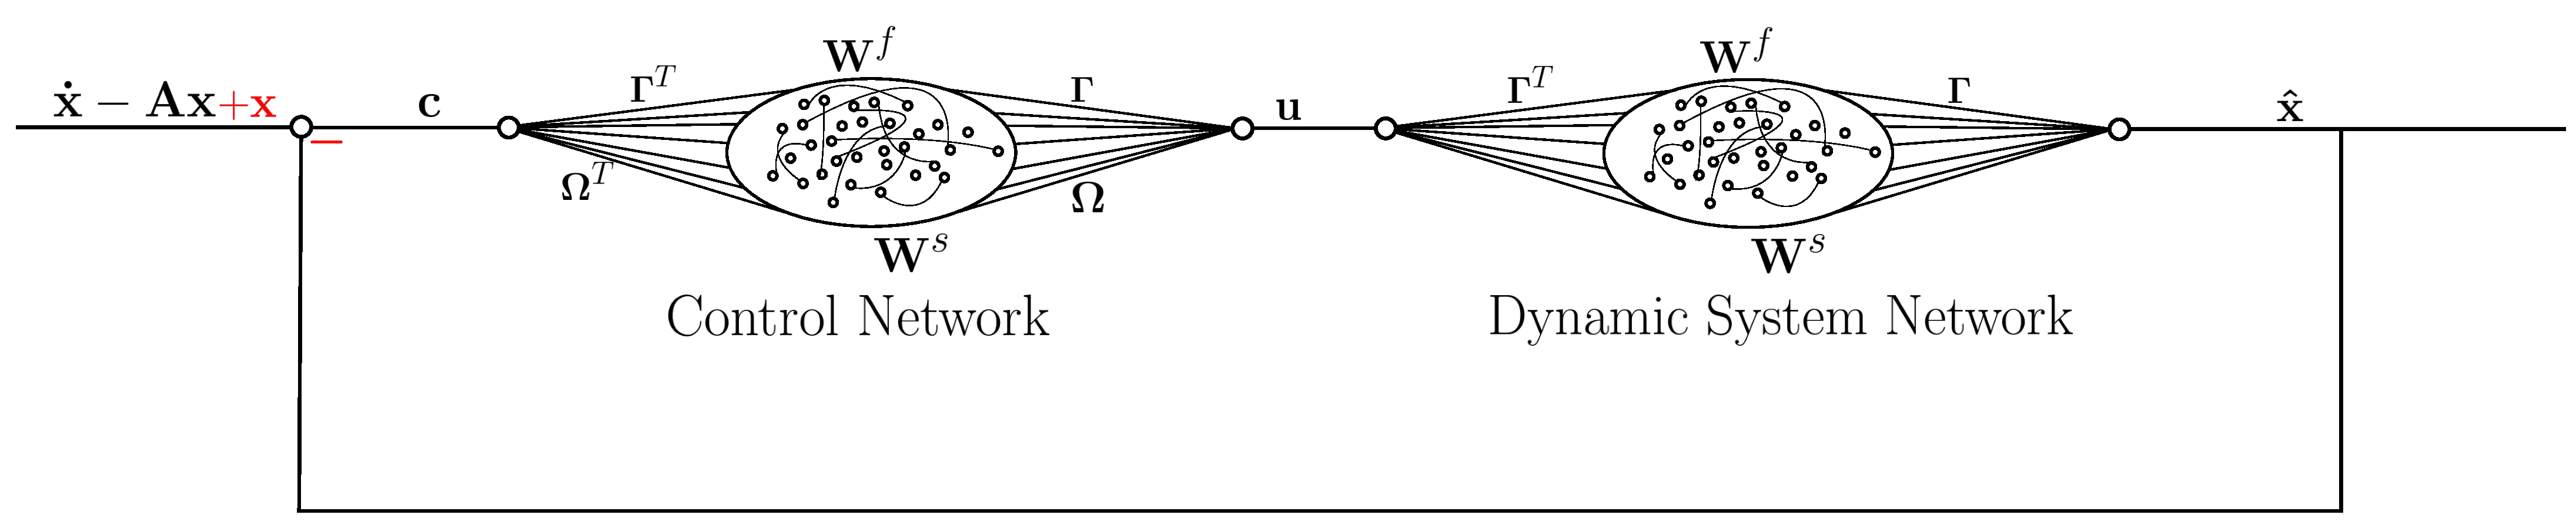
\includegraphics[width=\textwidth]{svg-inkscape/schematic_controller_network_feedback_2_nets.pdf}
		\caption{Add an extra loop to introduce feedback into the control network.}
		\label{fig:schematic_feedback_control_2_nets}
	\end{subfigure}
	\vfill{1cm}
	\begin{subfigure}{\textwidth}
		\centering
		\includegraphics[width=\textwidth]{../../plots/everything/feedback_2_nets.pdf}
		\caption{Comparison of control for our model problem with the controlling and simulating network with and without feedback. Both runs used networks with 50 neurons and identical parameters. Plots for $x_1$ and $x_2$ separately.}
		\label{fig:feedback_control_2_nets_error}

	\end{subfigure}
	\caption{Top: Schematic to the addition of feedback in the in the control network. Additions are highlighted in red. Bottom: Resulting improvement of error with the feedback loop added.}
\end{figure}
While this improves performance, as seen in \cref{fig:feedback_control_2_nets_error}, the network output is still unusable due to the error. Thus, efficient tracking is only possible using the analytically calculated matrices $\bmu{W}^f$ and $\bmu{W}^s$ and therefore disqualifies this approach as we aim to use the learned matrices.\\ Additionally, it was not possible to find training rules that would allow the training of the matrices used in the control network, posing further problems for our goal of using learning rules for the entire scheme.

\subsection{Merging two Networks}
Unfortunately, the use of feedback did not help to achieve acceptable results. It is therefore necessary to make a trade-off between biologic plausibility and control scheme performance. The alternative option being a combined network, incorporating both control and simulation at the same time.\\
As highlighted before, the governing force behind the control was not the network but rather only the definition of $\bmu{c}$. The network itself is primarily based around producing the necessary spikes and rates to return the corresponding control input $\bmu{u}$. Therefore, we construct a single network that handles both the control as well as the dynamic system itself. We define $\bmu{c}$ as
\begin{equation}
	\bmu{c} =  \bmu{\dot{x}}-\bmu{Ax}
\end{equation}
as before in the control network. In the current state, no control matrix is incorporated in the network which means that the network assumes $\bmu{B} = \bmu{I}$ which will be addressed later.

\subsubsection{Working as an Open-Loop Controller}
To begin, we set a sine wave as our target. As can be seen in \cref{fig:all_open_sine_base}, the aforementioned control using $\bmu{c}$ appears to deliver good results using the optimal weights. Both state trajectories almost perfectly overlap the target. As seen before, similar to \cref{ssec:combining-2-network}, dynamics quickly diverge due to the imperfections in the learned matrices making it impossible for the open loop to properly control the system, leading to an almost complete loss of the target trajectory. Yet the output shows better tracking than the separate networks.
\begin{figure}
	\centering
	\includegraphics[width=\textwidth]{../../plots/everything/open_sine_base.pdf}
	\caption{Control results for the ideal and learned matrices $\bmu{W}^f$ and $\bmu{W}^s$ on a sine wave target. Top panel shows the $x_1$ state and bottom $x_2$. Matrices were trained for 1000 epochs using the previously studied optimal parameters.}
	\label{fig:all_open_sine_base}
\end{figure}
The error shown in \cref{fig:all_open_sine_base} is almost purely due to inaccuracies in $\bmu{W}^s$. If the control is rerun but instead the optimal $\bmu{W}^s$ are used with the learned $\bmu{W}^f$, greatly improved results can be obtained.\\
\begin{figure}
	\centering
	\includegraphics[width=\textwidth]{../../plots/everything/all_open_sine_base_ideal_Ws.pdf}
	\caption{Control results from \cref{fig:all_open_sine_base} but with only either $\bmu{W}^f$ or $\bmu{W}^s$ trained. Top panel shows the $x_1$ state and bottom $x_2$. Matrices were trained for 1000 epochs using the previously studied optimal parameters.}
	\label{fig:all_open_sine_base_ideal_Ws}
\end{figure}
In \cref{fig:all_open_sine_base_ideal_Ws} the results show that if the ideal $\bmu{W}^s$ is used, control accuracy is greatly improved. Small errors still accumulate over time. These are from the remaining error in $\bmu{W}^f$ that is caused by small errors from training but also because $\bmu{W}^f$ adapts to the potential errors in $\bmu{W}^s$ during training. The opposite configuration yields even worse results, proving the principal error contribution stems from $\bmu{W}^s$.\\
As before, the main problem is that due to the open loop design, very precise system information is necessary. With training, only a perturbed system $\bmu{A}' = \bmu{A} + \bmu{\varepsilon}$ of the system matrix is learned. Without state feedback, control over $\bmu{A}'$ produces different dynamics which cannot be compensated without state feedback. This limits the applicability of any learned matrices.
\subsubsection{Adding Feedback}
In order to build a more robust controller, we add feedback to the control scheme as done before. Although this can be done identically by adding the error term directly onto $\bmu{c}$, we can change the formulation here due to only one network being present.
While we still send add the target trajectory to $\bmu{c}$, we can move the feedback loop directly into the network. The network output is calculated by by $\bmu{\hat{x}} = \bmu{\Gamma r}$. Ignoring the subtraction, this value is then fed back into the network using the same weights using $\bmu{\Gamma}^T\bmu{c}$. It is therefore the same as keeping adding another matrix
\begin{equation}
\bmu{W}^e = -\bmu{\Gamma}^T\bmu{\Gamma}
\end{equation}
to the network dynamics. The negative sign accounts for the subtraction we ignored earlier. The adjusted network dynamics are illustrated in \cref{fig:schematic_feedback_control}.
\begin{figure}
	\centering
	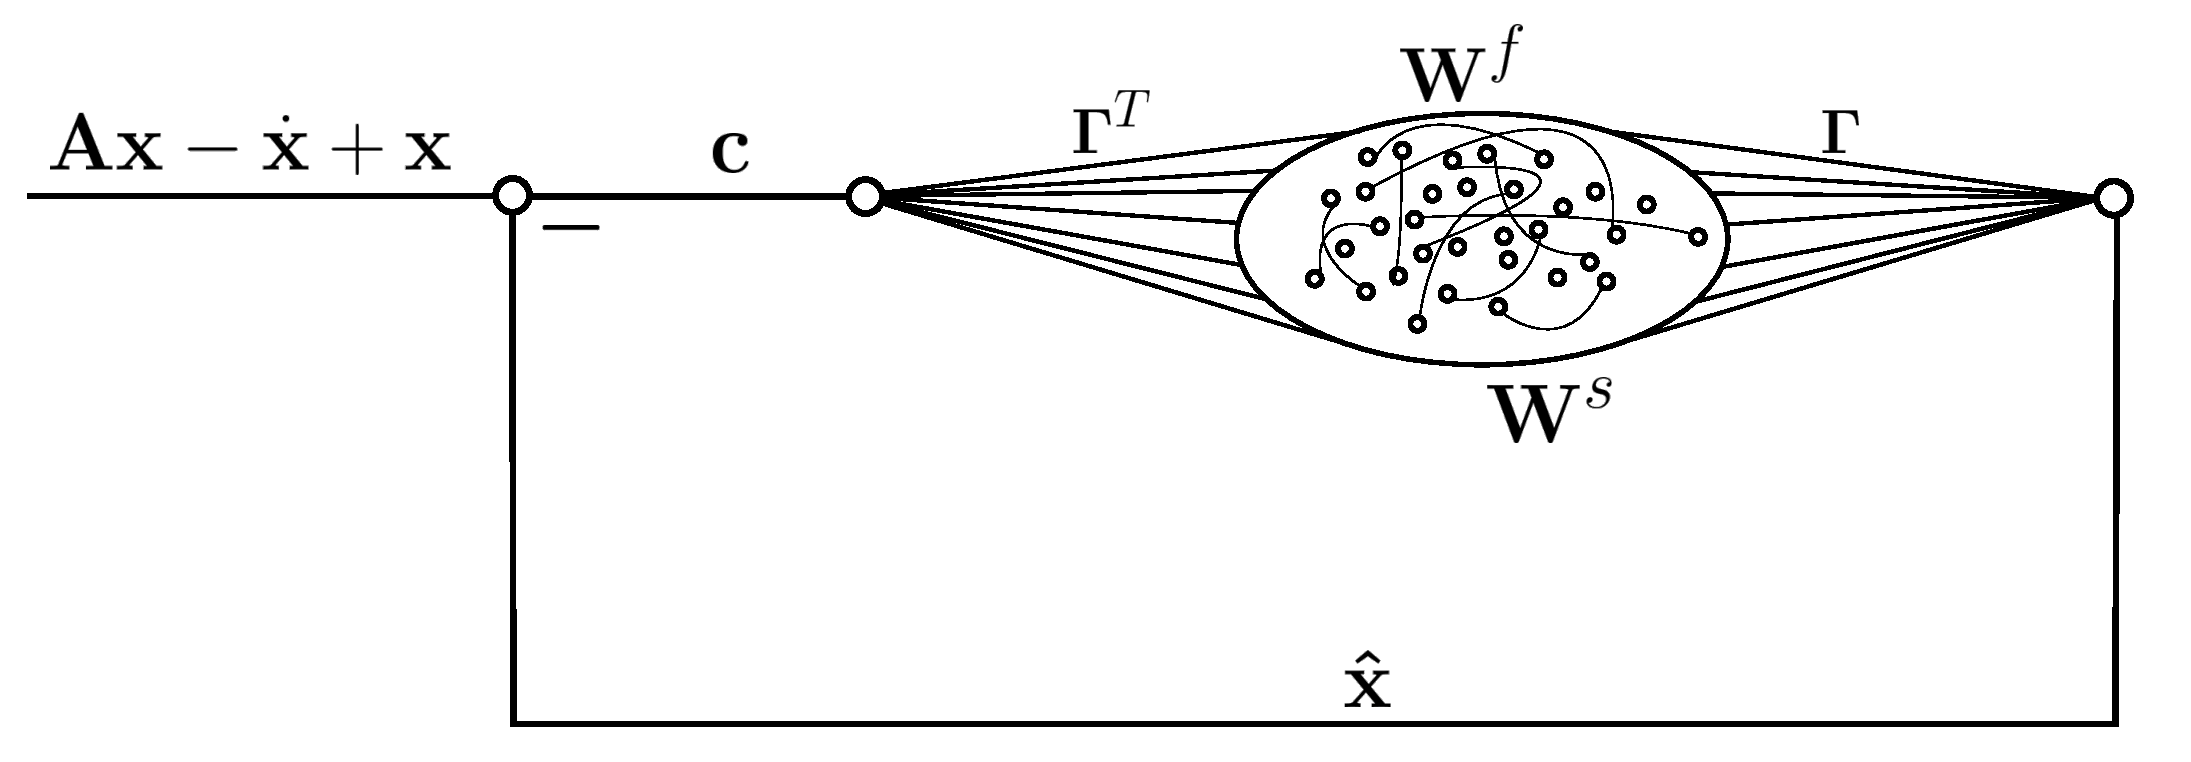
\includegraphics[width=\textwidth]{svg-inkscape/schematic_closed_loop_controller.pdf}
	\caption{Add an extra loop to introduce feedback into our control scheme. The outside loop can be integrated into the network similarly to $\bmu{W}^s$.}
	\label{fig:schematic_feedback_control}
\end{figure}
To measure its effectiveness, we run the simulation with the added matrix. In \cref{fig:all_closed_feedback_extra_loop}, we can clearly see the network performance is greatly improved. Both trajectories follow their target almost perfectly.
\begin{figure}
	\centering
	\includegraphics[width=\textwidth]{../../plots/everything/all_closed_sine_base.pdf}
	\caption{Control results from \cref{fig:all_open_sine_base} but with the added feedback loop seen in \cref{fig:schematic_feedback_control}.}
	\label{fig:all_closed_feedback_extra_loop}
\end{figure}

\subsubsection{Learning the New Feedback Loop}
Instead of introducing another matrix that is multiplied by the neuron firing rates, we can adjust the definition of $\bmu{W}^s$ to
\begin{equation}\label{eq:feedback_in_Ws}
\bmu{W}^s = \bmu{\Gamma}^T\left(\bmu{A} + (\lambda_d-1)\bmu{I} \right)\bmu{\Gamma}.
\end{equation}
This matrix can be further learned by the previous training algorithm by subtracting the identity matrix from $\bmu{A}$ before training.\\
We check if the learning of $\bmu{A-I}$ gives similar results to the case with the extra loop in \cref{fig:all_closed_feedback_extra_loop}. We retrain our model problem using the identical parameter set as before with the identity matrix subtracted.\\
To measure whether the training was able to reproduce the subtraction we calculate the inner matrix of \cref{eq:feedback_in_Ws} using regression.
\begin{equation}
	\bmu{M^*} = \min_{\bmu{M}} \| \bmu{\Gamma}^T\left(\bmu{M}+\lambda_d\bmu{I}\right)\bmu{\Gamma} - \bmu{W}^s\|_2^2
\end{equation}
It shows that in this test case the training was able to resolve the subtraction, with relative errors between matrix entries being less than 8\%.
In \cref{fig:all_closed_loop_learned} the result of training can be compared to the addition of the extra matrix after training. The final results is sufficiently accurate for almost perfect results. The target is tracked with almost identical performance as in \cref{fig:all_closed_feedback_extra_loop}.
\begin{figure}
	\centering
	\includegraphics[width=\textwidth]{../../plots/everything/all_closed_loop_learned.pdf}
	\caption{Control results from \cref{fig:all_closed_feedback_extra_loop} but with the added feedback loop learned and integrated into the network directly.}
	\label{fig:all_closed_loop_learned}
\end{figure}

\subsubsection{Restrictions on $\bmu{B}$}
All previous results are built on the implicit assumption of $\bmu{B} = \bmu{I}$. Although the results are acceptable, this assumption is prohibitively restrictive.\\
The easiest way to circumvent this restriction would be to have use the pseudo-inverse  $\bmu{B}^+$. If $\bmu{B}^+$ is available, the computations of network input can be simplified directly to
\begin{equation}\label{eq:feedback_with_B}
	\bmu{c} = \bmu{Bu}= \bmu{BB}^+\left(\bmu{\dot{x}- Ax}\right)
\end{equation}
if $\bmu{c} = \bmu{Bu}$ is substituted in the derivation of \cref{sec:simulation} and $\bmu{u} = \bmu{B}^+\left(\bmu{\dot{x} - Ax}\right)$,
ignoring the previously added feedback. But $\bmu{B}^+$ is often unavailable, moreover, biologically it is unrealistic to assume that the brain does matrix inversion. Instead, we restrict ourselves to matrices $\bmu{B}$ such that
\begin{equation}
	\bmu{BB}^+ = \bmu{BB}^T,
\end{equation}
which can be transformed to
\begin{equation}
\begin{aligned}
	\bmu{BB}^T &= \bmu{BB}^+\\
			  &= \bmu{B}\left(\bmu{B}^T\bmu{B}\right)^{-1}\bmu{B}^T\\
			  &\longrightarrow \bmu{B}^T\bmu{B} = \bmu{I}
\end{aligned}
\end{equation}
the condition that the Gram matrix of $\bmu{B}$ is the identity or the columns of $\bmu{B}$ form an orthonormal basis. The pseudo-inverse in \cref{eq:feedback_with_B} can then be replaced by $\bmu{B}^T$.\\

While this is again a strong limitation, it does increase the applicability of the network. To illustrate the this, we rerun the previous simulation with $\bmu{B} = [0,1]^T$ in \cref{fig:all_closed_1_net_with_b}.
\begin{figure}
	\centering
	\includegraphics[width=\textwidth]{../../plots/everything/1_net_feedback_with_B.pdf}
	\caption{Control results from \cref{fig:all_closed_feedback_extra_loop} with the input matrix $\bmu{B} =[0,1]^T$.}
	\label{fig:all_closed_1_net_with_b}
\end{figure}
Unfortunately, the addition of $\bmu{B}$ ruins the network performance with the trained matrices. Again, this is mainly caused by inaccuracies in $\bmu{W}^s$, as the network shows perfect results in \cref{fig:all_closed_1_net_with_b} when both $\bmu{W}^s$ and $\bmu{W}^f$(\cref{fig:all_closed_1_net_with_b}) or just $\bmu{W}^s$(not shown) is computed analytically.\\
The main reason the network performs subpar is the addition of $\bmu{BB}^T$ towards the error signal introduced before. As can be seen from \cref{fig:all_closed_1_net_with_b}, the error is primarily concentrated in the $x_1$ state which is not directly accessible by neither the error signal nor the network input $\bmu{c}$ due to
\begin{equation}
	\bmu{BB}^T = \begin{bmatrix}
	0&0\\
	0&1\\
	\end{bmatrix}
\end{equation}
removing any potential control over $x_1$, causing small inaccuracies to let the network diverge over time.
\subsection{Limitations}
The main limitation of the approaches presented here is the learning accuracy of $\bmu{W}^s$.
Both presented approaches deliver good results with analytically computed matrix weights. Either of them is usable to control a system if $\bmu{W}^s$ calculated analytically.\\
Only if either $\bmu{B}$ or the learning is neglected, both approaches can perform accurately. Ignoring $\bmu{B}$ hugely limits the applicability of the whole network despite the accurate results. To the above mentioned limitations all the limitations of previous sections also apply. This concerns especially the application to bigger systems, random initialization of weights before training, or the choice of $\bmu{\Gamma}$.\\
The addition of the error signal is necessary in order to balance the network noise. Due to lack of feedback, it is impossible to be accounted for. Therefore inherent noise in the network is completely unchecked.
Noise can alternatively be mitigated by scaling $\bmu{\Gamma}$ and the subsequent threshold to small scales. In this case, the number to spikes to represent the same signal will be increased, reducing the relative importance of spikes caused by noise. By doing this, the network is basically converted into a classic rate network.\\

\chapter{<Conclusions>}
Describe the conclusions (reflect on the whole introduction given in Chapter 1).

Discuss the positive effects and the drawbacks.

Describe the evaluation of the results of the degree project.

Describe valid future work.

The sections below are optional but could be added here.

\section{Discussion}

Answer the questions of the problem!!!!\\

\subsection{Future Work}

Maybe different noise models.. Brown noise
Adjust the input such that the imbalance can be negated and training is faster.\\
find nonlinearity\\
end point control\\
Test if learning with lower amplitude towards the end can refine the performance even more.\\
\todo{Double rate adjustment. In epoch and overall epochs}

Further work:\\
Maybe learning methods to control nonlinear dynamic systems\\
Maybe we can even do the adverserial attack to try to screw with the network.\\
Implement this on neuromorphic hardware\\

\subsection{Final Words}

\listoftodos








% \include{content}

\newpage
\addcontentsline{toc}{chapter}{References}
\textbf{If you are using mendeley to manage references, you might have to export them manually in the end as the automatic ways removes the "date accessed" field}
\printbibliography


\newpage
\appendix
\newpage
\etocdepthtag.toc{mtappendix}
\etocsettagdepth{mtchapter}{none}
\etocsettagdepth{mtappendix}{subsection}
\etoctocstyle{1}{Appendix - Contents}
\tableofcontents
\newpage


\chapter{First Appendix}
This is only slightly related to the rest of the report


\chapter{Second Appendix}
this is the information


\newpage
% This is the last page of the document
\thispagestyle{empty}
\AddToShipoutPictureBG*{%]
    \AtPageLowerLeft{%
        
\includegraphics[width=1.0\paperwidth]{setup/img/kth-footer.png}
    }%
}

\PlaceText{20mm}{282mm}{\color{white}\fontsize{12}{0}\sffamily www.kth.se }


\end{document}
